% This LaTeX document needs to be compiled with XeLaTeX.
\documentclass[
  10
]{article}
\usepackage[margin=2cm,includehead=true,includefoot=true,centering,]{geometry}
\usepackage{xcolor}
\usepackage{ucharclasses}
\usepackage{hyperref}
\usepackage{amsmath,amssymb}
\usepackage{amsfonts}
\usepackage[version=4]{mhchem}
\usepackage{stmaryrd}
\usepackage{bbold}
\usepackage{polyglossia}
\usepackage{fontspec}
\usepackage{ctex}
\usepackage[export]{adjustbox}
\usepackage{tabularx}
\usepackage{booktabs}

\usepackage{setspace}
\setstretch{1.2}

\makeatletter
\@ifundefined{KOMAClassName}{% if non-KOMA class
  \IfFileExists{parskip.sty}{%
    \usepackage{parskip}
  }{% else
    \setlength{\parindent}{0pt}
    \setlength{\parskip}{6pt plus 2pt minus 1pt}}
}{% if KOMA class
  \KOMAoptions{parskip=half}}
\makeatother
\usepackage{longtable,booktabs,array}
\newcounter{none} % for unnumbered tables
\usepackage{multirow}
\usepackage{calc} % for calculating minipage widths
% Correct order of tables after \paragraph or \subparagraph
\usepackage{etoolbox}
\makeatletter
\patchcmd\longtable{\par}{\if@noskipsec\mbox{}\fi\par}{}{}
\makeatother
% Allow footnotes in longtable head/foot
\IfFileExists{footnotehyper.sty}{\usepackage{footnotehyper}}{\usepackage{footnote}}
\makesavenoteenv{longtable}
\usepackage{graphicx}
\makeatletter
\newsavebox\pandoc@box
\newcommand*\pandocbounded[1]{% scales image to fit in text height/width
  \sbox\pandoc@box{#1}%
  \Gscale@div\@tempa{\textheight}{\dimexpr\ht\pandoc@box+\dp\pandoc@box\relax}%
  \Gscale@div\@tempb{\linewidth}{\wd\pandoc@box}%
  \ifdim\@tempb\p@<\@tempa\p@\let\@tempa\@tempb\fi% select the smaller of both
  \ifdim\@tempa\p@<\p@\scalebox{\@tempa}{\usebox\pandoc@box}%
  \else\usebox{\pandoc@box}%
  \fi%
}
% Set default figure placement to htbp
\def\fps@figure{htbp}
\makeatother
\setlength{\emergencystretch}{3em} % prevent overfull lines
\providecommand{\tightlist}{%
  \setlength{\itemsep}{0pt}\setlength{\parskip}{0pt}}


\hypersetup{colorlinks=true, linkcolor=blue, filecolor=magenta, urlcolor=cyan,}
\urlstyle{same}

\usepackage{colortbl}
\definecolor{table-row-color}{HTML}{999999}
\definecolor{table-rule-color}{HTML}{999999}
%\arrayrulecolor{black!40}
\arrayrulecolor{table-rule-color}     % color of \toprule, \midrule, \bottomrule
\setlength{\aboverulesep}{0pt}
\setlength{\belowrulesep}{0pt}


\setotherlanguages{english}
\IfFontExistsTF{Source Han Serif CN}
{\newfontfamily\chinesefont{Source Han Serif CN}}
{\IfFontExistsTF{Noto Serif CJK SC}
  {\newfontfamily\chinesefont{Noto Serif CJK SC}}
  {\IfFontExistsTF{SimSun}
    {\newfontfamily\chinesefont{SimSun}}
    {\IfFontExistsTF{FangSong}
      {\newfontfamily\chinesefont{FangSong}}
      {\newfontfamily\chinesefont{Arial Unicode MS}}
}}}
\IfFontExistsTF{Times New Roman}
{\newfontfamily\englishfont{Times New Roman}}
{\IfFontExistsTF{Liberation Serif}
  {\newfontfamily\englishfont{Liberation Serif}}
  {\IfFontExistsTF{DejaVu Serif}
    {\newfontfamily\englishfont{DejaVu Serif}}
    {\newfontfamily\englishfont{Arial}}
}}


\author{}
\date{}

\begin{document}


\section{Accurate multi-step wind and solar power forecasting based on
multi-scale convolutional Kolmogorov-Arnold network and improved
Lemming-optimized attention
fusion}\label{accurate-multi-step-wind-and-solar-power-forecasting-based-on-multi-scale-convolutional-kolmogorov-arnold-network-and-improved-lemming-optimized-attention-fusion}

\pandocbounded{
\includegraphics[keepaspectratio,alt={image}]{images/8c4c31793b88c00ac362a56da73704d13341f66a71a341fd4ce67df4359679ea.jpg}}

Siyuan Chen a , Hang Wan a,* , Botao Peng b , Rui Quan a , Yufang Chang
a , William Derigent c

a Hubei Key Laboratory for High-efficiency Utilization of Solar Energy
and Operation Control of Energy Storage System, Hubei University of
Technology, Wuhan, 430068, China

b Institute of Computing Technology, Chinese Academy of Sciences,
Beijing, 100190, China

c CRAN, CNRS UMR 7039, University of Lorraine, Vandœuvre-les-Nancy
Cedex, 54516, France

\section{A R T I C L E I N F O}\label{a-r-t-i-c-l-e-i-n-f-o}

Keywords:

Renewable energy management

Multi-step power forecasting

Multi-scale convolutional Kolmogorov-Arnold network

Artificial Lemming Algorithm

Efficient additive attention

\section{A B S T R A C T}\label{a-b-s-t-r-a-c-t}

With the deepening of power market reform, the increasing share of wind
and solar energy introduces significant challenges for power system
stability due to the high volatility and uncertainty of
weather-dependent generation. Accurate multi-step ultra-short-term
forecasting is therefore essential for ensuring power balance and
effective dispatch coordination in smart grids. To address this issue,
we propose a novel hybrid deep learning framework that integrates a
multi-scale convolutional Kolmogorov-Arnold network (MCKAN) to improve
forecasting performance. This network is specifically designed to
capture high-dimensional spatial and temporal features across multiple
levels of abstraction. To improve feature selection and scale-specific
weight allocation, we integrate an Efficient Additive Attention (EAA)
mechanism, which is applied for the first time in the context of
renewable energy forecasting. In addition, a Chaotic Quasi-Reverse
Artificial Lemming Algorithm (CQALA) is proposed to automatically
optimize the complex multivariate hyperparameters, enabling optimal
hyperparameter selection and improving the model's overall predictive
performance. Extensive experiments on a two-year wind and photovoltaic
power dataset from the State Grid of China demonstrate that the proposed
method outperforms several state-of-the-art models. For multi-step
forecasting, the mean absolute error is reduced by up to 27.6 percent
for photovoltaic power and 33.4 percent for wind power, highlighting the
practical value of the proposed approach in real-world renewable energy
management.

{\def\LTcaptype{none} % do not increment counter
\begin{longtable}[]{@{}|l|l|l|l|@{}}
\toprule\noalign{}
\endhead
\bottomrule\noalign{}
\endlastfoot
\hline
\multicolumn{2}{@{}l}{%
Nomenclature} & MCKAN & Multi-scale Convolutional Kolmogorov-Arnold
Network \\
\hline
\multicolumn{2}{@{}l}{%
Acronyms} & MCNN & Multi-scale Convolutional Neural Network \\
\hline
Adam & Adaptive Moment Estimation & MLP & Multilayer Perceptron \\
\hline
Air\_H & Relative Humidity & NP & Neural Prophet \\
\hline
Air\_P & Atmosphere & PSO & Particle Swarm Optimization \\
\hline
Air\_T & Air Temperature & PV & Photovoltaic \\
\hline
ALA & Artificial Lemming Algorithm & Q, K, V & Query, Key, Value \\
\hline
ARMA & Autoregressive Moving Average & RF & Random Forest \\
\hline
BPNN & Back Propagation Neural Network & RNN & Recurrent Neural
Network \\
\hline
CA & CosAttention & WD\_x & Wind Direction at height of x meters
(continued on next column) \\
\hline
\end{longtable}
}

(continued )

{\def\LTcaptype{none} % do not increment counter
\begin{longtable}[]{@{}|l|l|l|l|@{}}
\toprule\noalign{}
\endhead
\bottomrule\noalign{}
\endlastfoot
\hline
CKAN & Convolutional Kolmogorov-Arnold Networks & WP & Wind Power \\
\hline
CNN & Convolutional Neural Network & WS\_x & Wind Speed at height of x
meters \\
\hline
COA & Coati Optimization Algorithm & SVM & Support Vector Machine \\
\hline
CQALA & Chaos Quasi-opposition-based Artificial Lemming Algorithm & TSI
& Total Solar Irradiance \\
\hline
DNI & Direct Normal Irradiance & 3D-CNN & The Two-dimensional
Convolutional Neural Networks \\
\hline
EAA & Efficient Additive Attention & 2D-CNN & The Three-dimensional
Convolutional Neural Networks \\
\hline
EWMA & Exponentially Weighted Moving Average & & \\
\hline
& & & (continued on next page) \\
\hline
\end{longtable}
}

E-mail address: hang.wan@hbut.edu.cn (H. Wan).

(continued )

{\def\LTcaptype{none} % do not increment counter
\begin{longtable}[]{@{}|l|l|l|l|@{}}
\toprule\noalign{}
\endhead
\bottomrule\noalign{}
\endlastfoot
\hline
GA & Genetic Algorithm & Symbols & \\
\hline
GBDT & Gradient Boosting Decision Tree & MAE & Mean absolute error
(MW) \\
\hline
GHI & Global Horizontal Irradiance & NRMSE & Normalized Root Mean
Squared Error (NRMSE) \\
\hline
KANs & Kolmogorov--Arnold Networks & MAPE & Mean Absolute Percentage
Error (\%) \\
\hline
LSTM & Long Short-Term Memory & R2 & Coefficient of Determination \\
\hline
\end{longtable}
}

\section{1. Introduction}\label{introduction}

The growing scarcity of fossil fuel resources, combined with increasing
environmental concerns and international climate commitments, has
accelerated the global transition toward cleaner and more sustainable
energy systems (Kruitwagen et al., 2021; Raza et al., 2025). Among
various renewable energy sources, wind and solar power have emerged as
the most promising due to their high efficiency and environmental
benefits (He et al., 2025). According to the International Energy Agency
(International Energy Agency, 2024), by 2030, renewables will account
for half of global electricity generation, with wind and solar
photovoltaics contributing \(3 0 \%\) and solar capacity driving
\(8 0 \%\) of new installations. However, the integration of wind and
solar energy into the grid presents significant challenges due to their
inherent intermittency and weather dependence (Wan et al., 2025). These
characteristics lead to fluctuations in power output, complicating grid
planning, dispatching, and real-time operation (Li et al., 2024a).

To address these challenges, the integration of artificial intelligence
(AI) techniques into power forecasting has emerged as a key enabler for
effective and intelligent renewable energy management (Li et al., 2024b;
Moreno et al., 2024). This improvement in forecasting accuracy not only
enhances system reliability and cost-effectiveness, but also contributes
to reducing carbon emissions through more efficient energy scheduling
(Toghyani and Saadat, 2024; Ibrahim, 2023). Based on forecast horizons,
PV/Wind power forecasting is generally categorized into
ultra-short-term, short-term, medium-term and long-term forecasts
(Yaghoubirad et al., 2023). While medium-term and long-term forecasts
support site selection and capacity planning, and short-term forecasts
assist in day-ahead scheduling, ultra-short-term forecasts are critical
for real-time operational control, particularly in regions with high
renewable penetration. With the increasing integration of variable
renewables like wind and solar, power systems are becoming more volatile
at sub-hourly scales (Zhang et al., 2023). This has elevated
ultra-short-term forecasting to a central focus in power system
research, given its importance in maintaining real-time balance and
reliability.

In this context, this study aims to improve ultra-short-term power
forecasting using hybrid deep learning algorithms, in order to
facilitate real-time dispatch and enhance the operational reliability of
power systems with high renewable energy penetration. To ensure
real-time applicability, most publicly available power generation
datasets adopt a sampling interval of 5--15 min (Limouni et al., 2023).
Based on this temporal resolution, single-step forecasting predicts
power output one interval ahead and plays a critical role in preventing
short-term power shortages (Sun et al., 2023). However, its limited
predictive horizon restricts its effectiveness in supporting operational
dispatch and transmission planning decisions.

Building on the foundation of single-step forecasting, multi-step
forecasting extends the prediction horizon from 15 to 45 min or more,
thereby enabling more comprehensive and proactive decision-making in
power system operations (Zhang et al., 2024; Jin et al., 2025). While
one-step forecasting (15 min ahead) supports real-time power control,
two-step forecasting (30 min ahead) facilitates advance dispatch
planning and spinning reserve allocation, and three-step forecasting (45
min ahead) enables adjustments to inter-regional transmission schedules.
By

effectively capturing short-term fluctuations in renewable energy
output, multi-step forecasting improves resource allocation, enhances
system stability, and increases operational flexibility. In this
context, this study investigates advanced methods for multi-step
ultra-short-term forecasting to support real-time decision-making in
renewable-integrated power systems. The main contributions of this paper
are as follows:

\begin{enumerate}
\def\labelenumi{(\arabic{enumi})}
\item
  A multi-scale convolutional model, MCKAN, is proposed to improve
  multi-step ultra-short-term forecasting of wind and solar power by
  capturing multi-dimensional features across abstraction levels.
\item
  The efficient additive attention mechanism EAA is integrated into the
  hybrid deep learning model for the first time in renewable energy
  forecasting, enabling improved feature selection, weight allocation,
  and overall predictive performance.
\item
  To overcome manual hyperparameter tuning, the Chaotic Quasi-Reverse
  Artificial Lemming Algorithm (CQALA) is proposed. It leverages chaotic
  mapping and quasi-inverse learning to dynamically optimize kernel
  sizes and output units, improving accuracy and generalization.
\item
  The effectiveness and superiority of the proposed model in both
  single-step and multi-step forecasting are validated through
  comprehensive comparisons with state-of-the-art methods on a two-year
  wind and solar power dataset from the State Grid of China.
\end{enumerate}

The rest of this paper is organized as follows. Section 2 presents the
literature review and discuss the advantages and limitations of related
work. Section 3 introduces the foundational components and provides a
detailed description of the proposed method. Section 4 describes the
dataset and evaluation metrics used in the experiments. Section 5
presents the experimental results and performance analysis of the
proposed models. Section 6 discusses the limitations and outlines
potential directions for future research.

\section{2. Literature review}\label{literature-review}

Accurate forecasting of wind and solar power generation has become a
critical research area in renewable energy integration. Existing
forecasting methods are typically divided into three types: physical
models, statistical models, and artificial intelligence-based approaches
(Aslam et al., 2021). The traditional physical model approach simulates
the operation of wind and solar power generation systems based on
physical laws and meteorological data. Its core is to describe the
working principle of wind and solar power generation by establishing a
complex physical model, thus predicting the output of wind and solar
power (Dolara et al., 2015). However, this approach demands a large
amount of data during model establishment and debugging, and the
operation process is time-consuming. It is frequently used for long-term
prediction (Wolff et al., 2016); The statistical model approach is
primarily based on historical data. It predicts wind and solar power
generation through statistical analysis or time-series models, such as
Autoregressive Moving Average (ARMA), Exponentially Weighted Moving
Average (EWMA) (Almeida et al., 2017). While statistical methods are
easy to implement, their reliance on idealized assumptions during the
calculation process makes it challenging to capture the complex
nonlinear relationships and spatiotemporal dynamics of wind and solar
power generation systems (Lindig et al., 2018).

In recent years, deep learning, an important branch of artificial
intelligence, has shown excellent performance in renewable energy power
prediction (ElRobrini et al., 2024). Among them, Recurrent Neural
Networks (RNNs) have attracted significant attention for their ability
to process time-series data. Their memory mechanism allows RNNs to
capture temporal dependencies and utilize historical data, thereby
enhancing prediction accuracy (Abdel-Nasser and Mahmoud, 2019).

However, RNNs are susceptible to the gradient vanishing problem when
processing long sequences. This issue restricts their ability to capture
long-term dependencies and diminishes performance in tasks requiring
extended temporal context. Meanwhile, the success of Convolutional
Neural Networks (CNNs) in image processing has driven interest in
exploring their potential applications in time-series analysis (Ren et
al., 2025). CNNs extract local features from time-series data by
leveraging their local perception and hierarchical learning
capabilities. Their multi-layered architecture allows them to capture
complex patterns and improve prediction accuracy. Traditional CNN models
depend heavily on their local connection architecture and fixed-weight
mechanism. This reliance confines the receptive field to a narrow local
range, limiting the model's ability to adapt flexibly to dynamic data
changes (Hou et al., 2025).

To address these limitations, researchers have improved CNNs by
integrating techniques like multi-scale feature extraction and dynamic
time warping. For instance, Zhu et al.~(2021) introduced a wind-speed
prediction model based on a three-dimensional convolutional neural
network with behavioral feature learning. Ren et al.~(2022) proposed a
four-core deep CNN. In which, the CNN model was composed of a set of
convolutional modules with different kernel sizes to achieve high
prediction accuracy in photovoltaic power prediction. Chung et
al.~(2022) presented a parallel convolutional neural network (MCNN)
model for thermal load prediction, demonstrating superior performance
compared to other models. While the MCNN improves feature extraction
flexibility through a multi-branch structure, it significantly increases
the number of parameters required for its design. This leads to high
computational complexity and low training efficiency. To address these
challenges, Convolutional Kolmogorov--Arnold Networks (CKANs) were
proposed in (Bodner et al., 2024). By leveraging the Kolmogorov-Arnold
representation theorem (Liu et al., 2024), CKAN decomposes
high-dimensional functions into combinations of low-dimensional
functions. This reduces the number of parameters, enhances the model's
ability to capture global features, and significantly boosts prediction
accuracy. Consequently, prediction models based on CKANs show great
potential for complex and multi-dimensional wind and solar power
forecasting.

Single models frequently encounter challenges like overfitting and
limited interpretability. Some researchers have explored hybrid models
that integrate physical, statistical, and artificial intelligence
methods, leveraging the strengths of each approach while addressing the
weaknesses of single models (Devaraj et al., 2021). Xing et al.~(2024)
employed the KAN-Transformer hybrid model for ultra-short-term
wind-power prediction. This model exhibits superior prediction
performance compared to various advanced methods. Li et al.~(2024c) put
forward a multi-step wind-speed prediction hybrid model, namely a hybrid
model combining a Convolutional Neural Network and a Long Short-Term
Memory neural network (LSTM). Bashir et al.~(2025) introduced a hybrid
CNN-Transformer-MLP model that integrates CNN for local feature
extraction and Transformer-MLP for modeling long-term dependencies,
demonstrating superior performance over CNN, BiLSTM, and Transformer
baselines in wind and solar forecasting. Recent successes of hybrid
models in wind and solar forecasting highlight their effectiveness in
capturing complex temporal patterns. Therefore, multi-scale composite
models such as CKANS may serve as a viable and promising approach to
further enhance predictive performance.

In order to capture more complex dependencies and improve
representational power, attention mechanisms are often integrated into
hybrid deep learning architectures (Liu and Mao, 2024). Nguyen-Duc et
al.~(2024) proposed a multi-dimensional convolutional neural network
integrated with a Laplacian Attention for short-term photovoltaic power
prediction. Jonathan et al.~(2024) present a CNN-based hybrid model
enhanced with an attention mechanism. The attention module adaptively
assigns weights to different segments of the input, helping the model
focus on key information while suppressing noise, thereby improving
predictive performance. Shaker et al.~(2023).

introduce the Efficient Additive Attention (EAA) mechanism, which
demonstrates outstanding performance in visual applications. Unlike
conventional self-attention mechanisms, EAA avoids computationally
intensive matrix multiplications, thereby mitigating bottlenecks in
real-time processing and enabling deployment on devices with limited
computational resources. Additionally, EAA can be integrated into all
stages of the network, enhancing context information capture and
improving the balance between speed and accuracy (Hu et al., 2025).
Considering the need for efficient and accurate time-series data
processing in multi-step prediction, and the high sensitivity of hybrid
models to parameter settings, integrating EAA is expected to further
enhance their performance.

Although hybrid models offer significant advantages in improving
prediction accuracy, their complex structures and diverse designs
increase the challenges of parameter optimization (Bischl et al., 2023;
Quan et al., 2024a). Yu et al.~(2023) employed the Whale Optimization
Algorithm (WOA) to optimize the hyperparameters of the BiLSTM model,
enhancing its ability to capture complex temporal patterns for
photovoltaic power forecasting. Houran et al.~(Abou Houran et al., 2023)
applied the Coati Optimization Algorithm (COA) to tune CNN-LSTM
hyperparameters, improving model convergence speed and predictive
accuracy in offshore wind power forecasting. Quan et al.~(2024b)
utilized the Dung Beetle Optimization (DBO) algorithm for hyperparameter
tuning, effectively boosting the performance of the SATCN-BiLSTM hybrid
model for ultra-short-term PV power prediction.

However, some optimization algorithms suffer from issues such as a
tendency to fall into local optimality during the search process, poor
robustness, and sensitivity to initial conditions (Liu, 2025). To
address this issue, Xiao et al.~(2025) proposed the Artificial Lemming
Algorithm (ALA), a novel meta-heuristic inspired by the survival
behavior of lemmings. ALA effectively alleviates premature convergence
and enhances global search capability by maintaining a dynamic balance
between exploration and exploitation.

In summary, existing studies on wind and solar power forecasting based
on hybrid deep learning models have made significant progress in
improving prediction accuracy through various architectural innovations
and optimization techniques. However, accurate multi-step forecasting
remains constrained by challenges in multi-dimensional feature
extraction and hyperparameter tuning, especially under complex,
high-variability conditions. To address these issues, the next chapter
introduces a novel hybrid modeling framework designed to enhance feature
representation, focus attention on key information, and adaptively
optimize model parameters, thereby improving both accuracy and
generalization.

\section{3. Proposed methodology}\label{proposed-methodology}

To further enhance the performance of hybrid models in multi-step
renewable energy forecasting, this section presents the proposed deep
learning framework as shown in Fig. 1. The framework is composed of
three main components: the multi-scale convolutional network MCKAN for
hierarchical feature extraction, the Efficient Additive Attention EAA
for adaptive feature weighting, and the novel Chaotic Quasi-Reverse
Artificial Lemming Algorithm CQALA for dynamic hyperparameter
optimization. In the following subsections, each component is described
in detail, followed by a comprehensive explanation of the information
flow within the overall framework.

\section{3.1. Convolutional Kolmogorov-Arnold
network}\label{convolutional-kolmogorov-arnold-network}

Traditional multilayer perceptron architectures involve complex
operations and require a large number of parameters. These
characteristics limit their suitability for parallel computing in
large-scale neural networks. To address these limitations,
Kolmogorov--Arnold Networks have been proposed as an alternative to
traditional MLPs. It is inspired by the Kolmogorov--Arnold
representation theorem (Liu et al., 2024),

\pandocbounded{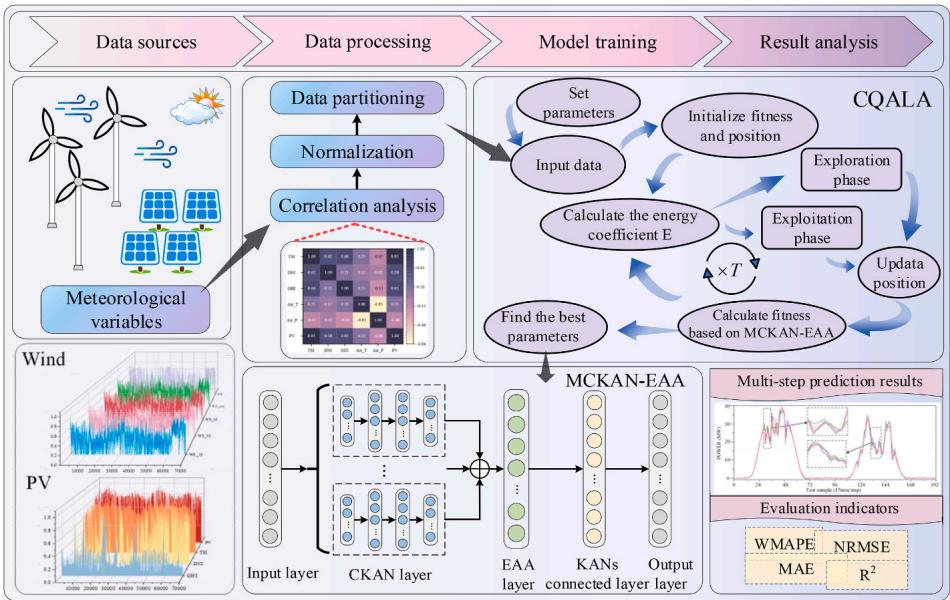
\includegraphics[keepaspectratio,alt={image}]{images/0a8c1ded0f17f2ff9316d71668c7719752f6cbdae0264484a13434a3e91dcdea.jpg}}

Fig. 1. The framework of proposed multi-step forecasting method.

which states that any multivariate continuous function can be expressed
as a finite superposition of continuous single-variable functions over
two layers. This provides a theoretical foundation for using KANs to
model complex, high-dimensional nonlinear relationships.

In the KANs network, for any continuous multivariable continuous
function \(f : [ 0 , 1 ] ^ { n } {  } R\) defined on a bounded domain,
there exists a positive integer \(2 n + 1\) such that the function can
be represented as shown in Equation (1). Each weight parameter is
modeled as a one-dimensional function parameterized by a spline. This
design allows the network to dynamically adapt its internal
representations based on the characteristics of the input data, thereby
enhancing flexibility and adaptability at the single-connection level.
Moreover, KANs employ learnable activation functions along the network
edges, in contrast to the fixed activation functions used in
conventional neural networks. This edge-based mechanism enhances the
model's ability to capture nonlinearities and data-specific behaviors.
The outputs of individual nodes are subsequently aggregated via
summation to produce accurate function approximations.

\[
f \left(\boldsymbol {x} _ {1}, \boldsymbol {x} _ {2}, \dots , \boldsymbol {x} _ {n}\right) = \sum_ {q = 1} ^ {2 n + 1} \Phi_ {q} \left(\sum_ {p = 1} ^ {n} \varnothing_ {q, p} \left(\boldsymbol {x} _ {p}\right)\right) \tag {1}
\]

\[
\Phi = \left\{\varnothing_ {q, p} \right\}, p = 1, 2, \dots n _ {\text {i n}}, p = 1, 2, \dots n _ {\text {o u t}} \tag {2}
\]

Where n represents the number of input variables. Both
\(\varPhi _ { q }\) and \(\textstyle \bigcirc _ { q , p }\) are
learnable one-sided functions. \(n _ { i n }\) and \$ \{ n \_ \{ o u t
\} \}\$ denote the number of input features and output features of a
specific layer, respectively. Each layer of KANs is constructed as a
learnable one-dimensional function matrix
\(\left\{ \emptyset _ { q , p } \right\}\) according to formula (2). The
internal function constitutes a KANs layer with \(n _ { i n } = n\) and
\(n _ { o u t } = 2 n + 1\) , while the external function defines a KANs
layer with \(n _ { i n } = 2 n + 1\) and \(n _ { o u t } = 1\) . The
activation function \(\mathcal { O } _ { q , p }\) within this
one-dimensional function matrix is linearly composed of the basis
function \(\mathbf { b } ( \mathbf { x } )\) and the spline function
spline(x). The activation function is defined as:

\[
\varnothing_ {q, p} (\boldsymbol {x}) = w _ {b} b (\boldsymbol {x}) + w _ {s} s p l i n e (\boldsymbol {x}) \tag {3}
\]

\[
b (x) = \frac {x}{1 + e ^ {- x}} \tag {4}
\]

\[
\operatorname {s p l i n e} (x) = \sum_ {i} c _ {i} B _ {i} (X) \tag {5}
\]

Where, \(w _ { b }\) and \(w _ { s }\) are learnable weights used to
control the overall size of the activation function, \(c _ { i }\) is a
trainable coefficient, and \(B _ { i } ( X )\) represents the b-spline
function. Therefore, the network structure of KANs is mapped using the
complex function of equations (6) and (7). Among them, each activation
function \(\mathcal { O } _ { l , j , i }\) represents a spline.

\[
K A N (x) = \left(\Phi_ {L - 1} ^ {*} \Phi_ {L - 2} ^ {*} \dots^ {*} \Phi_ {0}\right) x \tag {6}
\]

\[
X _ {i + 1} = \Phi_ {i} \left(\boldsymbol {x} _ {i}\right) = \left( \begin{array}{c c c} \varnothing_ {i, 1, 1} (\cdot) & \dots & \varnothing_ {i, 1, n _ {i}} (\cdot) \\ \vdots & \ddots & \vdots \\ \varnothing_ {i, n _ {i + 1}, 1} (\cdot) & \dots & \varnothing_ {i, n _ {i + 1}, 1} (\cdot) \end{array} \right) X _ {i} \tag {7}
\]

Similar to conventional CNNs, KAN-based convolutional layers perform
local computations using learnable kernels, but they are prone to
overfitting in deep architectures. To address this issue, the
Convolutional Kolmogorov--Arnold Network (CKAN) proposed in (Bodner et
al., 2024) replaces each kernel element with a nonlinear function based
on B-spline basis functions. This architecture enables the network to
extract complex representations through adaptive, nonlinear
convolutional kernels. These parameterized kernels effectively capture
intricate data dependencies while significantly reducing the number of
trainable parameters. The complete mathematical formulation of the
convolutional kernel is defined as follows:

\[
K A N K e r n e l = \left[ \begin{array}{l l} \varnothing_ {1 1} & \varnothing_ {1 2} \\ \varnothing_ {2 1} & \varnothing_ {2 2} \end{array} \right] \tag {8}
\]

\[
\phi_ {k, l} (\boldsymbol {x}) = \sum_ {m = 1} ^ {M} \theta_ {k, l, m} B _ {m} (\boldsymbol {x})
\]

Each \(\varnothing _ { k l }\) is a nonlinear function, and
\(\theta _ { k , l , m }\) is the weight of the basis function. The
convolution of the Convolutional Kolmogorov-Arnold Network is calculated
in a similar way to the traditional convolution, and its computation
formula is shown in equation (9).

\[
y (i, j) = \sum_ {k = 0} ^ {m - 1} \sum_ {l = 0} ^ {n - 1} \phi_ {k, l} (x (i - k, i - l)) \tag {9}
\]

where, \(m\) and \(n\) represent the height and width of the convolution
kernel respectively, and \(x ( i { - } k , i { - } l )\) represents the
value of the input data \(x\) at position \(( i - k , i - l )\) .

\section{3.2. Multi-scale convolutional Kolmogorov-Arnold
network}\label{multi-scale-convolutional-kolmogorov-arnold-network}

Since multi-step forecasting of wind and solar power generation imposes
higher demands on a model's ability to capture complex temporal dynamics
and intrinsic multi-scale patterns, this study extends the CKAN
framework and proposes the Multi-Scale Convolutional Kolmogorov--Arnold
Network. Motivated by the demonstrated effectiveness of convolutional
neural networks in extracting multi-scale features through convolutions
with varying kernel sizes (Wang et al., 2022; Cui et al., 2025), the
proposed MCKAN model adopts a parallel and hierarchical architecture to
extract temporal features across multiple scales. This design enables
the model to capture diverse temporal patterns more effectively and
better accommodate the complexity and variability inherent in sequential
data.

The structure of MCKAN is shown in Fig. 2. MCKAN adopts a multilayer
parallel convolutional architecture based on KANs. Each convolution
structure consists of an input layer, an output layer, a CKAN layer, and
a pooling layer. Within this architecture, large convolutional kernels
capture long-term, slowly evolving trends by spanning extended
historical periods. In contrast, small kernels extract short-term
fluctuations and transient patterns within narrow time windows. This
multi-scale design allows the model to effectively learn temporal
features at multiple levels of abstraction, thereby improving its
capacity to model the complexity and non-stationarity of sequential
data.

Specifically, once the raw meteorological data containing multiple
variables has been received and preprocessed, the input layer passes the
processed data to the parallel KAN-based convolutional layers. Each
branch operates over a specific temporal scale, as determined by the
size of its convolutional kernel, and applies dynamic nonlinear mapping
functions to short segments of the input time series. These operations
enable each branch to extract salient features that correspond to
distinct temporal dynamics. Among them, the adaptive capacity of the
KANbased convolutional layer plays a pivotal role in ensuring
representational continuity across multiple temporal resolutions. Its
internal dynamic grid expansion mechanism allows the model to
continuously adjust the domain of the spline basis functions based on
the changing input features. Therefore, the temporal consistency of
feature representations can be maintained even under highly
non-stationary and rapidly fluctuating eigenvalue structures, such as
those commonly found in meteorological data. This architectural design
significantly improves the model's robustness in modeling complex,
multi-scale temporal dependencies.

Subsequently, the pooling layer then down samples the feature maps to
reduce dimensionality and enhance translation invariance. The output
layer integrates features from the multi-layer parallel branches based
on the target task, generating a more comprehensive feature
representation. These structural components enable the model to
ultimately explore meteorological features across multiple time scales
in depth and accurately capture the dynamic changes of meteorological
data at different time dimensions.

\section{3.3. Efficient additive
attention}\label{efficient-additive-attention}

The attention mechanism plays a vital role in processing long-term
time-series data. It effectively captures contextual dependencies and
focuses on regions most relevant to the current time step. In other
words, it dynamically attends to critical information in the sequence,
thereby improving the model's ability to process complex temporal
patterns (Liu et al., 2021). However, conventional attention mechanisms
rely on matrix multiplications, which introduce substantial
computational overhead. These operations significantly increase
computational complexity and memory usage (Malhotra and Addis, 2024). To
address the aforementioned issues, the additive attention mechanism
replaces the dot-product operation used in traditional attention with
element-wise interactions. Building on this idea, an improved version
called Efficient Additive Attention (EAA) was proposed in (Shaker et
al., 2023). The process framework diagram of EAA is shown in Fig. 3.

This mechanism discards key-value interactions and solely focuses on
efficiently encoding query-key interactions through the merging of
linear projection layers. This improvement enables the mechanism to
maintain good performance while substantially reducing computational
complexity, leading to faster operation. The specific operation process
of this mechanism is as follows:

The Efficient Additive Attention (EAA) mechanism begins by taking the
input embedding matrix \(\ b X \in \ b R ^ { n \times d }\) , where
\(n\) is the token length and d is the embedding dimension. The input is
linearly projected using learnable weight matrices \(W _ { q }\) and
\(W _ { k }\) to generate the query and key matrices Query (Q) and Key
\(( K )\) , respectively, where \(Q , K \in R ^ { n \times d }\) . To
compute the attention distribution, the query matrix Q is multiplied by
a learnable weight vector \(\omega _ { \alpha } \in R ^ { d }\) ,
yielding the attention weights \(\alpha \in R ^ { n \times d }\) through
equation(10):

\[
\alpha = \frac {Q . w _ {a}}{\sqrt {d}}, a \in R ^ {n} \tag {10}
\]

These attention weights are then used to compute a global query vector
\(q \in R ^ { d }\) via weighted aggregation of the query tokens as in
(11). The contextual information is then captured by performing element-

\pandocbounded{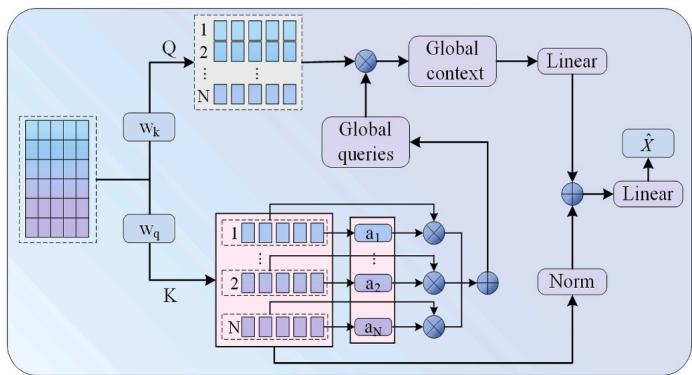
\includegraphics[keepaspectratio,alt={image}]{images/5862a8cca94e1f0f0afad121f2399cffe86f0de67552ae1c9014c8e09e972e51.jpg}}

Fig. 3. Architecture flowchart of EAA.

\pandocbounded{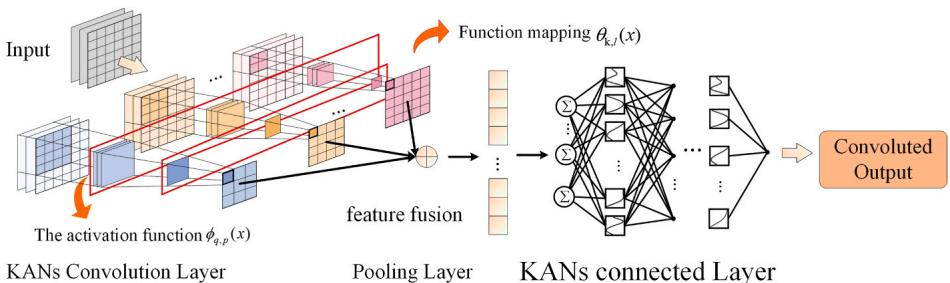
\includegraphics[keepaspectratio,alt={image}]{images/e2d0137299b931d358aecdadaed721d5bbc584f267e19e4351ef4a96e45e4cbc.jpg}}

Fig. 2. The structure of MCKAN.

wise multiplication between the global query vector \(q\) and the key
matric K, resulting in a global context representation
\(C \in R ^ { n \times d }\) as follows:

\[
q = \sum_ {i = 1} ^ {n} a _ {i} ^ {*} Q _ {i}, q \in R ^ {d} \tag {11}
\]

\[
C = K \circ q \tag {12}
\]

Where, ∘ denotes broadcasted element-wise multiplication. This operation
encodes the interaction between each key token and the global query,
effectively modeling the global context with linear complexity. Finally,
a linear transformation layer is used to realize the interaction between
the query matrix Q and the key matrix K to learn the hidden
representation of the tokens. The output \(\widehat { x }\) of the
additive attention is calculated as shown in equation (13):

\[
\widehat {x} = \widehat {Q} + T \left(K ^ {*} q\right) \tag {13}
\]

By avoiding costly query-key dot products and key-value matrix
multiplications, EAA achieves attention computation using only linear
projections and element-wise operations. This simplified yet effective
formulation allows EAA to capture global contextual dependencies while
maintaining high computational efficiency. Moreover, its lightweight
structure makes it easy to apply across all layers of the network,
including those handling longer token sequences.

\section{3.4. The proposed Chaos Quasi-opposition-based Artificial
Lemming
Algorithm}\label{the-proposed-chaos-quasi-opposition-based-artificial-lemming-algorithm}

To improve the robustness of multivariate parameter optimization in
hybrid forecasting models, this paper proposes the Chaotic Quasi-Reverse
Artificial Lemming Algorithm (CQALA). The algorithm is inspired by the
collective survival strategies of lemmings, which are small Arctic
rodents known for their adaptive behavior in extreme environments. From
a biological perspective, lemmings exhibit two primary behavioral
phases. The exploration phase includes long-distance migration and
digging tunnels to locate new habitats. The exploitation phase involves
foraging for food and evading natural predators. These behavioral
mechanisms contribute to maintaining population diversity and
adaptability under environmental pressures.

Inspired by these behaviors, CQALA constructs a mathematical model that
integrates chaotic mapping, quasi-reverse learning, and adaptive
survival strategies to enhance optimization performance. As

shown in Fig. 4, the algorithm starts by defining the search space
boundaries and applying chaotic quasi-reverse initialization to improve
population diversity. During each iteration, CQALA evaluates the fitness
of each individual and updates their positions accordingly. A key
feature of CQALA is the introduction of an energy factor E, which
dynamically balances exploration and exploitation based on the current
system state. This mechanism promotes more efficient convergence toward
the global optimum.

Upon reaching the maximum number of iterations, CQALA outputs the
optimal set of hyperparameters for the hybrid model. The following
sections present a detailed explanation of each component strategy
within the CQALA framework.

\section{(a) Initialization}\label{a-initialization}

The initialization of ALA is similar to that of other metaheuristic
algorithms, starting from the initial population position. The initial
population position Z is a matrix with N rows and D columns, where N
represents the number of populations and D represents the dimension of
the solution space. Its calculation method is shown in Equation (14).

\[
\vec {Z} _ {i} = \vec {L} + \vec {r} \times (\vec {U} - \vec {L}), i = 1, 2, \dots , N \tag {14}
\]

where, \(\overrightarrow { U }\) and
\(\stackrel { \longrightarrow } { L }\) represent the algorithm search
upper and lower bounds, respectively, and \(\overrightarrow { r }\) is a
random vector in the interval {[}0,1{]}. Enhancing the initialization
strategy in an optimization algorithm has a direct impact on its
performance. A well-designed initialization strategy can significantly
increase population diversity and reduce the algorithm's sensitivity to
initial solutions (Li et al., 2021). Therefore, optimizing the
initialization process is essential to ensuring robust algorithm
performance in complex optimization tasks. This paper adopts an improved
initialization strategy based on chaotic quasi-reverse learning. By
leveraging the unpredictability and ergodicity of chaotic systems, the
strategy incorporates quasi-reverse solutions to generate a diverse and
well-distributed initial population.

\section{(b) Tent Chaos Map}\label{b-tent-chaos-map}

Chaotic mapping, based on sensitive initial conditions, generates
chaotic initial sequences, which are used to enhance population
diversity and local search in optimization algorithms (Tian, 2017).
Among various chaotic mappings, the Tent map has received particular

\pandocbounded{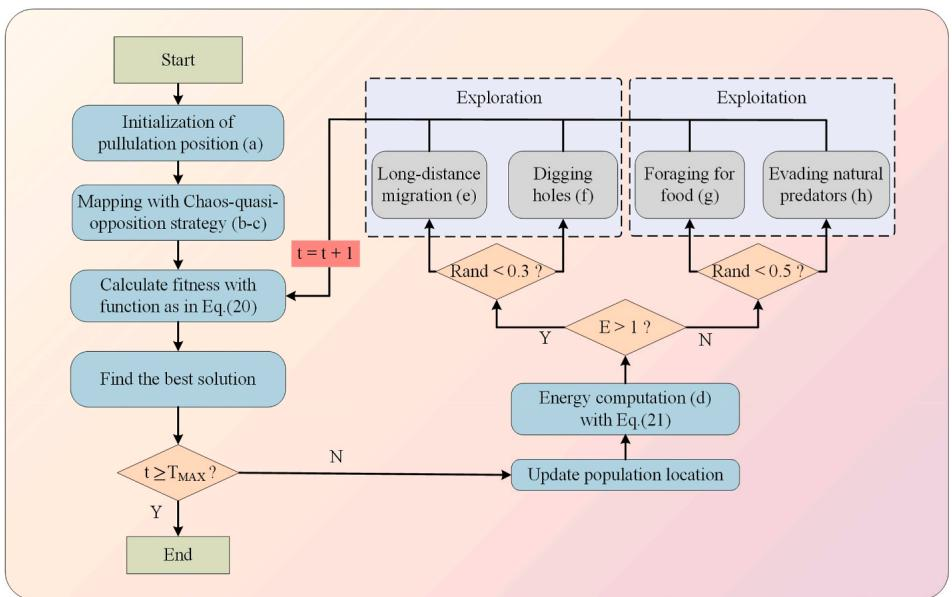
\includegraphics[keepaspectratio,alt={image}]{images/c1dda24f6ccb940e6d0f5b73fa477538dc224ebfb7e169cf3e5f5deab3674f07.jpg}}

Fig. 4. Flowchart of CQALA.

attention due to its simple mathematical formulation and strong chaotic
characteristics (Qi et al., 2024). The Tent map is capable of generating
highly random and ergodic chaotic sequences. These sequences are mapped
to the solution space to generate a well-distributed initial population,
thereby enhancing the algorithm's global search ability and stability.
The iterative formula of the Tent map is provided in Equation (15), and
the mapping of chaotic sequences to the optimization problem's solution
space is mathematically defined in Equation (16).

\[
y _ {i + 1, d} = \left\{ \begin{array}{c} \frac {y _ {i , d}}{a}, y _ {i, d} <   a \\ \frac {1 - y _ {i , d}}{1 - a}, y _ {i, d} \geq a \end{array} \right. \tag {15}
\]

\[
\overrightarrow {Z} _ {i} = \overrightarrow {L} + y _ {i, d} \times (\overrightarrow {U} - \overrightarrow {L}), i = 1, 2, \dots , N \tag {16}
\]

where, a is a custom control parameter. At the same time, in order to
maintain its chaotic characteristics, the initial value
\(y _ { 1 , d }\) cannot be equal to \(a\) .

\section{(c) Introducing Quasi-opposition-based
learning}\label{c-introducing-quasi-opposition-based-learning}

To further enhance the diversity of the introduced population, this
paper presents a quasi-reverse learning mechanism (Kundu and Garg,
2025). This mechanism calculates the reverse solution for each initial
solution within the search space and combines these reverse solutions
with the original initial solutions. The calculation method for the
reverse solutions is presented in Equations (17) and (18). The selected
position is a random number between the mid-value of the upper and lower
bounds and the reverse position. Incorporating this randomness
facilitates the exploration of potential high-quality solution regions
in the search space that might be overlooked by the original solutions.

\[
\overrightarrow {\widehat {Z} _ {i} ^ {o}} = \overrightarrow {L} + \overrightarrow {U} - \overrightarrow {Z} _ {i} \tag {17}
\]

\[
\overrightarrow {\widehat {Z} _ {i} ^ {q \theta}} = r a n d \left(\frac {\overrightarrow {L} + \overrightarrow {U}}{2}, \overrightarrow {\widehat {Z} _ {i} ^ {o}}\right) \tag {18}
\]

\[
f _ {i} = \text {f i t n e s s - f u n c i t o n} (\text {p a r a m s}, x, y) \tag {20}
\]

Where params decodes the hyperparameters of deep learning modes, (e. g.,
learning rate, number of hidden units, dropout rate), the value \(x\)
and y are the training set (train x, train Y) and validation set (val x,
val Y) in the case of power forecasting. Since the goal is to minimize
the prediction error, the lower the RMSE, the higher the fitness of the
corresponding hyperparameter set. This fitness value guides the ALA
search process toward optimal hyperparameter combinations that yield
better forecasting performance.

\section{(d) Energy coefficient calculation for strategy
selection}\label{d-energy-coefficient-calculation-for-strategy-selection}

To ensure a stable transition between exploration and exploitation
phases, the ALA incorporates an energy factor that applies from the
initial exploration phase to the subsequent exploitation phase. The
mathematical formulation of this energy factor is presented in Equation
(21). When the of energy factor \(E > 1\) , the ALA enters the
exploration phase, characterized by long-distance migration and
resource-seeking behavior. As the iteration count rises, the value of E
will gradually decline until \(E \leq 1\) . At this point, the ALA can
smoothly transition from the exploration phase to the exploitation
phase, which involves foraging and predator-avoidance activities.

\[
E (t) = 4 \times \arctan \left[ 1 - \frac {t}{T _ {\max}} \right] \times \ln \left(\frac {1}{\text {r a n d}}\right) \tag {21}
\]

\section{(e) Long-distance migration}\label{e-long-distance-migration}

Lemmings, a rodent species with the highest reproductive capacity
globally, are prone to food shortages in their populations due to
overbreeding. Therefore, to survive, some lemmings migrate long
distances to find a more suitable habitat. The direction and distance of
this longdistance migration are influenced by multiple factors,
including environmental and biological ones. The mathematical
representation of this behavior is as follows:

\[
\overrightarrow {Z} _ {i} (t + 1) = \overrightarrow {Z} _ {\text {b e s t}} (t) + F \times \overrightarrow {B M} \times \left(\overrightarrow {R} \times \left(\overrightarrow {Z} _ {\text {b e s t}} (t) - \overrightarrow {Z} _ {i} (t)\right)\right) + \left(1 - \overrightarrow {R}\right) \times \left(\overrightarrow {Z} _ {i} (t) - \overrightarrow {Z} _ {a} (t)\right) \tag {22}
\]

where, \(r a n d ( a , b )\) represents a random number between a and b.
The original initial population and the reverse population are merged,
sorted and selected according to the fitness value, and finally the
individual with the best fitness is selected as the final initial
population. The matrix expression of the final initial population
position \({ \widehat { Z } } _ { q o }\) is as follows:

\[
\widehat {Z} _ {q o} = \left[ \begin{array}{c} \widehat {Z} _ {1} ^ {q o} \\ \widehat {Z} _ {2} ^ {q o} \\ \vdots \\ \widehat {Z} _ {i} ^ {q o} \\ \vdots \\ \widehat {Z} _ {N} ^ {q o} \end{array} \right] = \left[ \begin{array}{c c c c c c} x _ {1, 1} & x _ {1, 2} & \dots & x _ {1, j} & \dots & x _ {1, D} \\ x _ {2, 1} & x _ {2, 2} & \dots & x _ {2, j} & \dots & x _ {2, D} \\ \vdots & \vdots & \ddots & \vdots & \ddots & \vdots \\ x _ {i, 1} & x _ {i, 2} & \dots & x _ {i, j} & \dots & x _ {i, D} \\ \vdots & \vdots & \ddots & \vdots & \ddots & \vdots \\ x _ {N, 1} & x _ {N, 2} & \dots & x _ {N, j} & \dots & x _ {N, D} \end{array} \right] j = 1, 2, \dots , D \tag {19}
\]

To evaluate the quality of each candidate solution (i.e., a set of
hyperparameters) generated by the Artificial Lemming Algorithm, a
fitness function is designed based on the model's predictive performance
on a validation dataset:

where, \(\vec { Z } _ { i } ( t )\) and \(\vec { Z } _ { i } ( t + 1 )\)
represent the population positions at this moment and the next moment
respectively, \(\overrightarrow { Z } _ { b e s t } ( t )\) represents
the current optimal solution, \(\overrightarrow { Z } _ { a } ( t )\)
represents the position of an individual randomly selected from the
population, a is an integer value in the interval {[}1,N{]}, and \(F\)
is used as a sign to change the search direction to jump out of the
local optimum. Its mathematical expression is shown in equation (23).
\(\overrightarrow { B M }\) is a random number variable that
characterizes Brownian motion. Brownian motion has a dynamic and uniform
step size, which helps to fully explore the solution space. The standard
Brownian motion step size is obtained by the probability function of the
standard normal distribution represented by equation (24).
\(\xrightarrow [ { R } ] { }\) is a random vector whose element value
range is in the interval {[}-1,1{]}, which is used to regulate the
movement of individuals in the population and to characterize the
interaction between individuals. Its mathematical expression is shown in
equation (25). where, \(\lfloor { } ^ { * } \rfloor\) is the floor
function, and rand represents a random number between the interval
{[}0,1{]}.

\[
F = \left\{ \begin{array}{c c} 1 & \text {i f} \lfloor 2 \times \operatorname {r a n d} + 1 \rfloor = 1 \\ - 1 & \text {i f} \lfloor 2 \times \operatorname {r a n d} + 1 \rfloor = 2 \end{array} \right. \tag {23}
\]

\pandocbounded{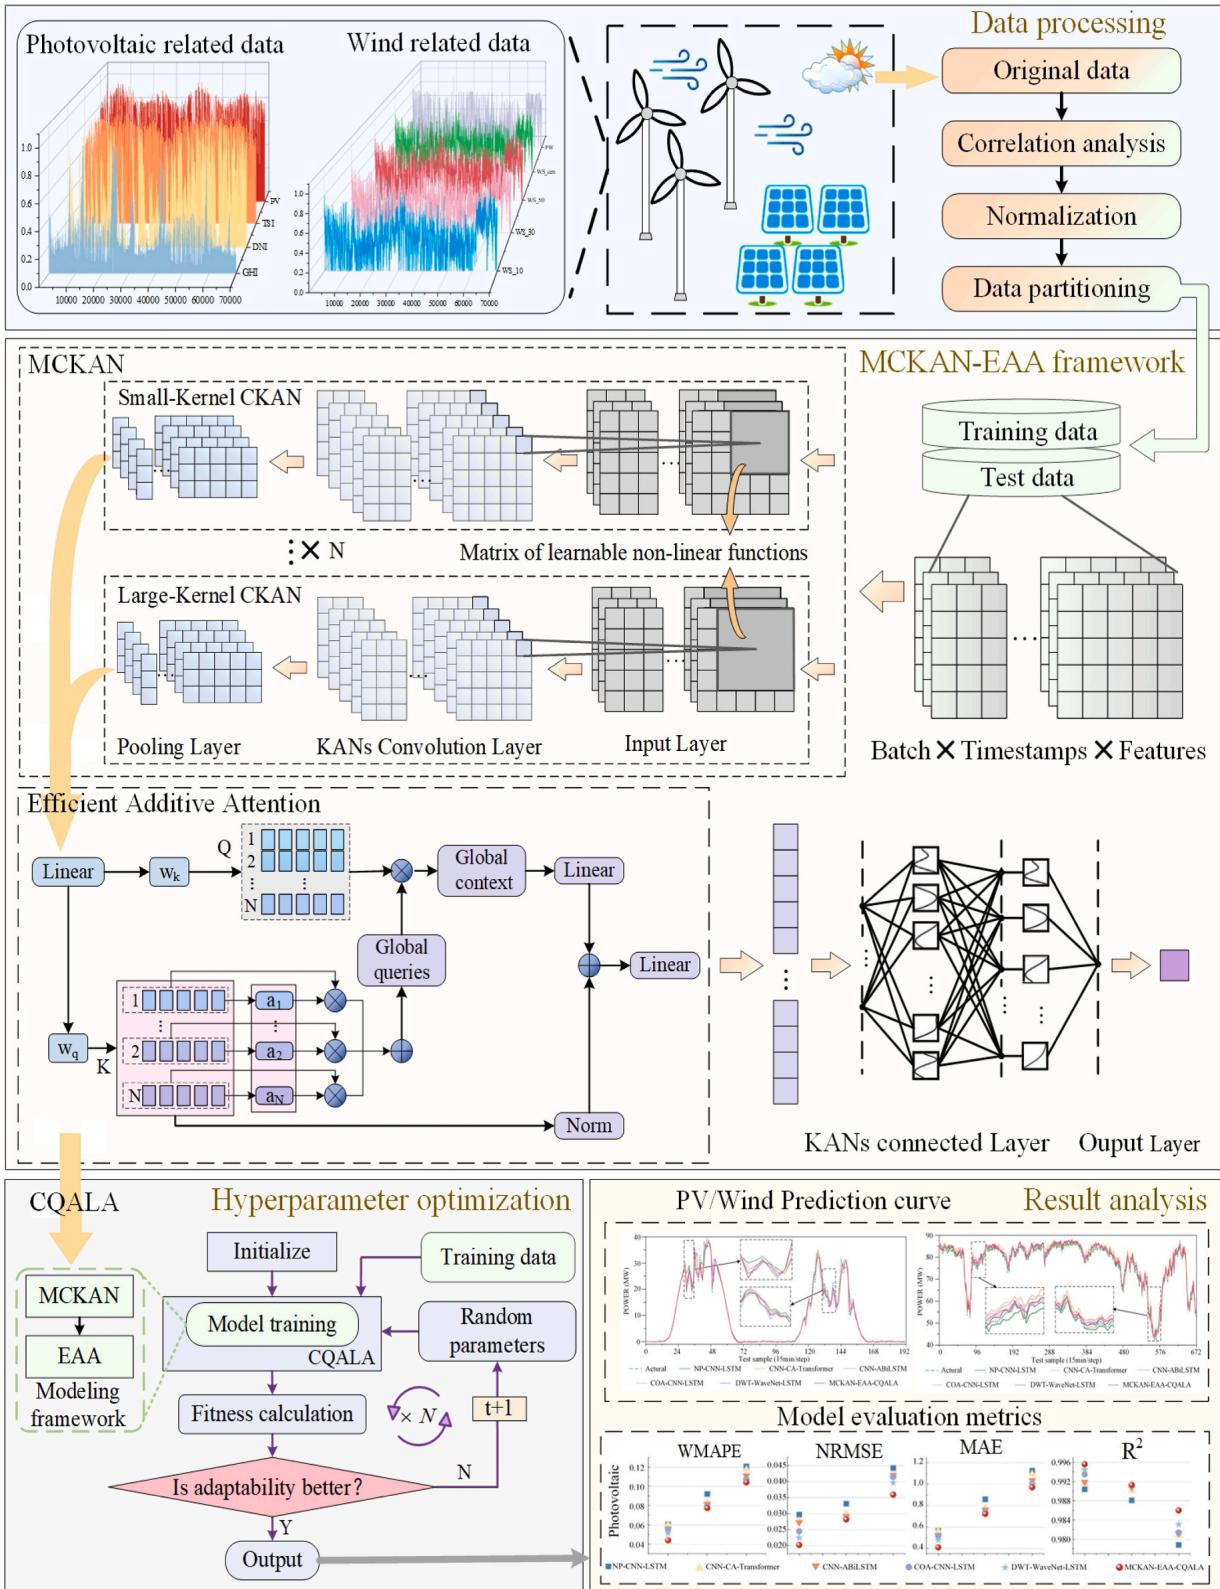
\includegraphics[keepaspectratio,alt={image}]{images/7a1ea1cbaae14132f49b680d08229de91c7a17c4e39ef40521918a652cb2319c.jpg}}

Fig. 5. Overall flowchart of the proposed MCKAN-EAA-CQALA.

\[
f _ {B M} (x; 0, 1) = \frac {1}{\sqrt {2 \pi}} e ^ {- \frac {x ^ {2}}{2}} \tag {24}
\]

\[
\overrightarrow {R} = 2 \times \operatorname {r a n d} (1, D) - 1 \tag {25}
\]

\section{(f) Digging holes}\label{f-digging-holes}

Lemmings dig complex tunnels and burrows in snow and underground for
survival. These structures help them avoid predators and store food.
Equation (26) models the behavior of burrow location selection.

\[
\overrightarrow {Z} _ {i} (t + 1) = \overrightarrow {Z} _ {i} (t) + F \times L \times \left(\overrightarrow {Z} _ {\text {b e s t}} (t) - \overrightarrow {Z} _ {b} (t)\right) \tag {26}
\]

where, \(\vec { Z } _ { b } ( t )\) represents the position of an
individual randomly selected from the population, b is an integer value
in the interval {[}1,N{]}, and L is a changing random number. Its
calculation formula is shown in (27).

\[
L = \operatorname {r a n d} \times \left(1 + \sin \left(\frac {t}{2}\right)\right) \tag {27}
\]

\section{(g) Foraging for food}\label{g-foraging-for-food}

Lemmings move randomly within the tunnels they have dug. They utilize
their acute sense of smell and hearing to locate food. The random
hunting behavior of lemmings in this area is modeled by a spiralwinding
mechanism. The corresponding equation is as follows:

\[
\overrightarrow {Z} _ {i} (t + 1) = \overrightarrow {Z} _ {\text {b e s t}} (t) + F \times \text {s p i r a l} \times \text {r a n d} \times \overrightarrow {Z} _ {i} (t) \tag {28}
\]

\[
\operatorname {s p i r a l} = \text {r a d i u s} \times (\sin (2 \pi \times \text {r a n d}) + \cos (2 \pi \times \text {r a n d})) \tag {29}
\]

\[
\text {r a d i u s} = \sqrt {\sum_ {j = 1} ^ {D} \left(Z _ {\text {b e s t} , j} (t) - Z _ {i j} (t)\right) ^ {2}} \tag {30}
\]

where, spiral represents the spiral shape in the process of searching
for food, and radius represents the radius of the search range for
foraging, that is, the Euclidean distance between the current solution
and the optimal solution.

\section{(h) Evading natural
predators}\label{h-evading-natural-predators}

Lemmings possess remarkable running capabilities. They frequently employ
deceptive maneuvers to evade predators and retreat into tunnels. The
formula for updating the position during this escape behavior is
presented in Equation (31).

\[
\overrightarrow {Z} _ {i} (t + 1) = \overrightarrow {Z} _ {\text {b e s t}} (t) + F \times G \times \operatorname {L e a y} (D) \times \left(\overrightarrow {Z} _ {\text {b e s t}} (t) - \overrightarrow {Z} _ {i} (t)\right) \tag {31}
\]

Where \(G\) represents the escape coefficient, which represents the
escape ability of lemmings, and its mathematical expression is shown in
equation (32). Leay(*) represents the leay flight function, and its
flight trajectory expression is shown in equation (33).

\[
G = 2 \times \left(1 - \frac {t}{T _ {\text {m a x}}}\right) \tag {32}
\]

\[
\operatorname {L e a y} (x) = 0, 0 1 \times \frac {u \times \sigma}{| v | ^ {\frac {1}{\beta}}} \tag {33}
\]

\[
\sigma = \left(\frac {\Gamma (1 + \beta) \times \sin \left(\frac {\pi \beta}{2}\right)}{\Gamma \left(\frac {1 + \beta}{2}\right) \times \beta \times 2 ^ {\left(\frac {\beta - 1}{2}\right)}}\right) ^ {\frac {1}{\beta}} \tag {34}
\]

Where, t and \(T _ { m a x }\) represent the current iteration number
and the maximum iteration number, \(u\) and \(\nu\) are random values
between the interval {[}0,1{]}, and \(\beta\) is a constant equal to
1.5.

\section{3.5. The proposed MCKAN-EAA-CQALA
model}\label{the-proposed-mckan-eaa-cqala-model}

The hybrid multi-prediction model framework proposed in this paper is
shown in Fig. 5, data preprocessing, which mainly includes three main
parts: data preprocessing, MCKAN-EAA framework, and CQALA Hyperparameter
optimization. In particular, the MCKAN model is responsible for feature
extraction and time-series prediction, while the EAA module focuses on
capturing and processing key information from the data. The CQALA
algorithm is employed to optimize the hyperparameters of the hybrid
model, thereby enhancing its prediction accuracy and convergence
stability. The overall process of the proposed multi-step prediction
method is as follows.

During data preprocessing, the original wind and solar power data
exhibited issues such as low quality and coarse feature granularity. To
address these challenges, Pearson correlation analysis was conducted to
identify meteorological variables that are strongly correlated with
power output and eliminate those with weak or no correlation. As
illustrated in the data processing section of Fig. 5, the variation
trends of features with strong correlations to power are visualized.
These selected high-correlation features are then normalized, and all
features are scaled to a consistent range to improve the stability and
convergence speed of model training. Finally, the normalized dataset is
split into training and testing sets, completing the data preprocessing
stage. The preprocessed data is subsequently fed into the hybrid
prediction framework, MCKAN-EAA-CQALA, for model training and
forecasting.

During the model training stage, the structure and workflow of the
hybrid prediction model MCKAN--EAA are described in detail. First, the
partitioned dataset is fed into the MCKAN module in the form of a
threedimensional tensor with the shape (Batch \(\times\) Timestamps
\(\times\) Features). MCKAN employs a multi-layer

parallel CKAN architecture to effectively extract complex
multidimensional features from the time series data of wind and solar
power generation. Each CKAN structure primarily consists of an input
layer, a KANs-based convolutional layer, and a pooling layer. The input
layer receives the formatted time series data and feeds it into multiple
parallel convolutional branches.

The KANs convolutional layer, as a key component for feature extraction,
captures complex temporal and spatial patterns by decomposing and
recombining the input data. This enables the model to significantly
reduce the number of parameters and computational complexity while
maintaining high representational capacity. The pooling layer applies a
sliding window mechanism to perform max pooling or average pooling
operations over local regions, enabling dimensionality reduction and
salient feature extraction. This process enhances the model's
generalization ability. As the final step in the feature extraction
process, MCKAN captures features at multiple scales and dimensions
through parallel convolutional branches with varying kernel sizes,
thereby providing high-quality feature representations for subsequent
time series modeling and optimization.

Subsequently, the MCKAN multi-step prediction model concatenates the
features extracted from each parallel convolutional branch and feeds the
fused feature vector into the Efficient Additive Attention module.
Within EAA, the concatenated features are first linearly transformed
into query (Q) and key (K) vectors. This transformation is performed
using a predefined linear mapping matrix and aims to project the
original

features into a new vector space, thereby enhancing their expressiveness
within the attention mechanism. Based on the constructed query and key
vectors, the EAA module computes attention weights and generates a
global query vector to enable global weighted interactions among
features. This mechanism allows the model to dynamically adjust the
importance of different features, thereby effectively capturing
potential dependencies and temporal associations. EAA then outputs a
fused feature representation based on additive attention, providing more
discriminative inputs for downstream modeling. Building on this, the
enhanced features are passed to the KANs combination layer, where they
undergo nonlinear transformation and restructuring through an efficient
KANs-based approximation and recombination mechanism. This further
improves the model's representational capacity for final prediction.

In the hyperparameter optimization stage, the Chaos
Quasiopposition-based Artificial Lemming Algorithm proposed is used to
automatically search for the optimal model parameters. Initially, CQALA
performs the initialization of hyperparameter settings and population
positions, and the preprocessed meteorological data is fed into the
model. After the initial round of model training, the algorithm
evaluates the objective function value for each individual in the
population, including the learning rate, number of hidden units, and
dropout rate, and selects the best-performing individual as the initial
global optimum. During the iterative optimization process, CQALA
simulates the survival strategy of lemmings by continuously exploring
the solution space and generating new candidate solutions through
dynamic updates of the individuals' positions. In each iteration, the
newly generated hyperparameter combination is fed into the MCKAN-EAA
model for training, and its performance is assessed using the objective
function. If the new solution outperforms the current global optimum,
the global best parameters are updated accordingly. Otherwise, only the
iteration state is updated, and the current best solution is retained.
This process continues until the predefined termination condition is
met.

Finally, the optimal hyperparameter configuration identified by CQALA is
used to retrain the MCKAN-EAA model. To assess its effectiveness,
comprehensive experiments are performed on wind and photovoltaic
datasets from the China Power Grid, with comparisons made against
state-of-the-art approaches. Evaluation metrics, including Weighted
Absolute Percentage Error (WAPE) and Mean Squared Error (MSE), are
employed to quantify performance, confirming the model's superiority in
prediction accuracy and stability.

\section{4. Data preparation}\label{data-preparation}

\section{4.1. Data sources}\label{data-sources}

The wind and solar power data used in this paper are sourced from the
historical data collected by the State Grid Corporation of China (Chen
and Xu, 2022). The original dataset spans a two-year period from January
1, 2019, to December 31, 2020, with a uniform 15-min time resolution,
resulting in a total of 70,176 data points. It includes six wind farms
with nominal capacities ranging from 36 to 200 MW (MW), and eight
photovoltaic (PV) power stations with nominal capacities between 30 and
130 MW. These sites are located across three major climate regions in
China: North China, Central China, and Northwest China. This broad
spatial distribution ensures substantial geographic and climatic
diversity in the dataset.

In this work, we focus on one wind farm and one PV power station located
in North China, a region characterized by strong seasonal variation,
including dry winters and convective weather in summer. These dynamic
conditions provide a representative and challenging testbed for
evaluating the robustness of short-term power forecasting models. The
selected wind farm has a nominal capacity of 96 MW and consists of 48
XE72 wind turbines, each with a rated capacity of
\(2 0 0 0 \mathrm { k W }\) , a hub height of
\(6 5 . 0 \mathrm { ~ m ~ }\) , and a rotor diameter of
\(7 0 . 7 \textrm { m }\) . The wind dataset contains power output (WP,
in MW) and relevant meteorological variables, including wind speed and
direction at 10 m, 30 m, 50 m, and nacelle

\pandocbounded{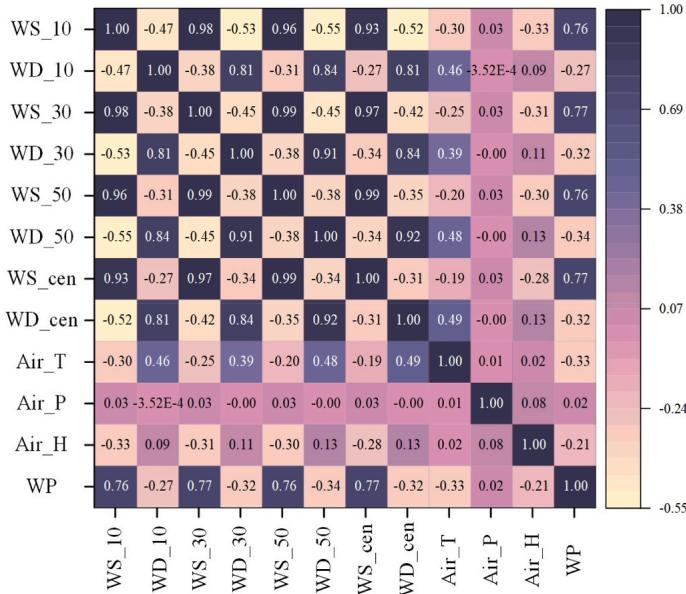
\includegraphics[keepaspectratio,alt={image}]{images/a110834c98af484c0d7176ac10792eca7cfe01be39437c56e31e131dd1da9c61.jpg}}

Fig. 6. Heat map based on Pearson correlation for WP prediction.

\pandocbounded{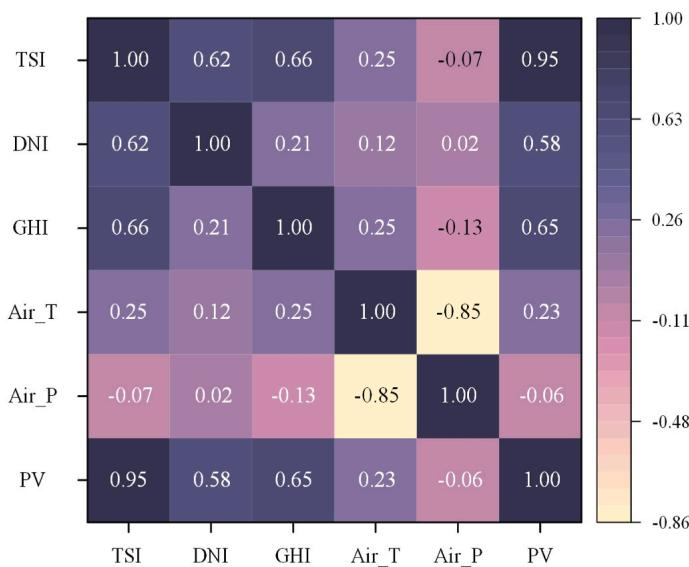
\includegraphics[keepaspectratio,alt={image}]{images/0448ca30a38b130d9f0f05e8dfd20e35fc6f1fef4bd8febd67ea9bfd80efd327.jpg}}

Fig. 7. Heat map based on Pearson correlation for PV prediction.

height (WS\_10, WD\_10, WS\_30, WD\_30, WS\_50, WD\_50, WS\_cen,
WD\_cen), air temperature (Air\_T), air pressure (Air\_P), and humidity
(Air\_H).

The selected PV station has a nominal capacity of 50 MW. The PV dataset
includes power output (PV, in MW) along with key solar irradiance and
weather variables: total solar irradiance (TSI), direct normal
irradiance (DNI), global horizontal irradiance (GHI), air temperature
(Air\_T), and air pressure (Air\_P).

\section{4.2. Data preprocessing}\label{data-preprocessing}

Since the original dataset publication has already provided detailed
specifications for handling missing values and outliers, this section
focuses on correlation analysis and Dataset splitting. To identify input
features that are most relevant to power prediction, the Pearson
correlation coefficient is used to quantify the linear relationship
between meteorological variables and power output (Buhan et al., 2016).
This allows the model to concentrate on informative inputs and avoid
redundant data. The calculation formula for the Pearson correlation

Table 1 Statistical information of Wind and PV power dataset.

{\def\LTcaptype{none} % do not increment counter
\begin{longtable}[]{@{}llllllllll@{}}
\toprule\noalign{}
\endhead
\bottomrule\noalign{}
\endlastfoot
\multirow{2}{*}{Dataset Information} & \multicolumn{5}{l}{%
Wind Dataset} & \multicolumn{4}{l@{}}{%
PV Dataset} \\
& WS\_10 & WS\_30 & WS\_50 & WS\_cen & Power & GHI & DNI & TSI &
Power \\
Average value & 5.04 & 6.62 & 7.44 & 8.15 & 28.76 & 67.69 & 93.26 &
266.21 & 9.67 \\
Maximum value & 15.28 & 19.71 & 21.81 & 23.82 & 114.36 & 989 & 980 &
1359,00 & 48.32 \\
Minimum value & 0 & 0 & 0 & 0 & 0 & 0 & 0 & 0 & 0 \\
Standard deviation & 2.76 & 3.28 & 3.59 & 3.80 & 28.01 & 111.2 & 200.78
& 367.89 & 13.71 \\
\end{longtable}
}

coefficient is as follow:

\[
r = \frac {\sum_ {t = 1} ^ {N} \left(x _ {t} - \bar {X}\right) \left(y _ {t} - \bar {Y}\right)}{\sqrt {\sum_ {t = 1} ^ {N} \left(x _ {t} - \bar {X}\right) ^ {2}} \sqrt {\sum_ {t = 1} ^ {N} \left(y _ {t} - \bar {Y}\right) ^ {2}}} \tag {35}
\]

Where, \(x _ { t }\) and \(y _ { t }\) represent the values of the
influencing variable and the predicted variable at time t, respectively.
Additionally, and \(\overline { { X } }\) and \(\overline { { Y } }\)
denote the average values of the influencing variable and the predicted
variable.

Figs. 6 and 7 respectively present the target variable (power
generation) and the correlation coefficients between each influencing
factor and the target for the wind and photovoltaic power datasets. In
Fig. 6, WS\_10, WS\_30, WS\_50, and WS\_cen show strong positive
correlations (above 0.7) with PW, while the remaining variables exhibit
weak correlation. Therefore, these four wind speed variables are
selected as input features for the wind power dataset.

For PV prediction as shown in Fig. 7, GHI, DNI, and TSI exhibit strong
positive correlations (greater than 0.5). Notably, TSI shows the highest
correlation, reaching 0.95. In contrast, ATM and AT display weak
correlations. Thus, GHI, DNI, and TSI are selected as input features for
the photovoltaic dataset. Detailed information on the selected input
features is provided in Table 1.

A large variation in the original data will affect the efficiency of
model training and the accuracy of prediction. To mitigate this issue,
all feature variables were normalized to a common scale prior to model
input. This preprocessing step reduced data variability and
significantly accelerated gradient descent convergence, thereby
improving model stability and interpretability (Singh and Singh, 2022).
Therefore, Min-Max Normalization is employed, a common and effective
data normalization method (Zhao et al., 2024), is employed to scale
feature data to the range {[}0, 1{]}. The mathematical expression is
given as follows:

\[
x ^ {\prime} = \frac {x - x _ {\text {m i n}}}{x _ {\text {m a x}} - x _ {\text {m i n}}} \tag {36}
\]

Where, \(x ^ { \prime }\) and \(x\) denote the normalized data and the
original data, respectively. Meanwhile, \(x _ { m a x }\) and
\(x _ { m i n }\) denote the maximum and minimum values of the original
data, respectively.

Appropriate data partitioning is essential for adequate model training.
Therefore, the normalized dataset is divided into a training set (56,238
samples) and a test set (13,939 samples) based on the commonly used
80:20 split ratio (Cui et al., 2024a). Sliding windows with a fixed
length are used to generate input sequences for the forecasting model. A
window of 96 time steps (covering the past \(2 4 \ \mathrm { h }\) at
15-min intervals) is applied to generate input features. A recursive
multi-step forecasting strategy is then used to predict power generation
15, 30, and 45 min ahead. The output data has the same time resolution
as the input.

\section{4.3. Evaluation indicators}\label{evaluation-indicators}

To assess the accuracy and broad applicability of model predictions,
this study employs four error indicators for performance assessment,
namely, Weighted Mean Absolute Percentage Error (WMAPE), Mean Absolute
Error (MAE), Normalized Root Mean Square Error (NRMSE)

and Coefficient of Determination \(( \mathbb { R } ^ { 2 } )\) . The
effectiveness of the proposed model's predictions will be evaluated
based on these performance metrics. In general, a lower value of MAE,
MSE, and RMSE, along with an \(\mathrm { R } ^ { 2 }\) value closer to
1, indicates better predictive performance of the model. The definitions
of these indicator are as follows:

Weighted Mean Absolute Percentage Error:

\[
W M A P E = \frac {\sum_ {t = 1} ^ {N} | X (t) - \widehat {X} (t) |}{\sum_ {t = 1} ^ {N} | X (t) |} \times 100 \% \tag{37}
\]

Mean absolute error:

\[
M A E = \frac {1}{N} \sum_ {t = 1} ^ {N} | X (t) - \widehat {X} (t) | \tag {38}
\]

Normalized Root Mean Square Error:

\[
N R M S E = \frac {\sqrt {\frac {1}{n} \sum_ {t = 1} ^ {n} \left(\mathcal {Y} _ {t} - \widehat {\mathcal {Y}} _ {t}\right) ^ {2}}}{\mathcal {Y} _ {\text {m a x}} - \mathcal {Y} _ {\text {m i n}}} \tag {39}
\]

Coefficient of Determination:

\[
R ^ {2} = 1 - \frac {\sum_ {I = 1} ^ {N} (X (t) - \widehat {X} (t)) ^ {2}}{\sum_ {I = 1} ^ {N} (X (t) - \bar {X} (t)) ^ {2}} \tag {40}
\]

Where, \(X ( t )\) and \(\widehat { X } ( t )\) denote the actual value
and the predicted value, respectively. \(\overline { { X } } ( t )\)
represents the mean of the samples, and \(N\) represents the number of
samples used for evaluation.

\section{5. Experimental results}\label{experimental-results}

\section{5.1. Parameter setting}\label{parameter-setting}

All simulations in this study are conducted using the Python programming
language within the Jupyter Notebook environment. The deep learning
model is implemented and optimized using the Tensor-Flow library under
Python 3.10. Experiments are carried out on a Matrix Origin cloud server
equipped with an NVIDIA Tesla V100 GPU (32 GB) and an Intel Xeon
Platinum 8260L CPU \(@\) 2.30 GHz. The detailed model parameters are
listed in Table 2.

The hyperparameters of the proposed model are carefully designed to
capture the multi-scale characteristics of wind and photovoltaic power
time series. In the MCKAN module, a hierarchical convolutional structure
is adopted, where Kernel Pool 1 = (Li et al., 2024b; Toghyani and
Saadat, 2024) with Dilation \(= 3\) , Kernel Pool \(2 =\) (Wan et al.,
2025; Li et al., 2024b) with Dilation \(= 2\) , and Kernel Pool \(3 =\)
(Kruitwagen et al., 2021; He et al., 2025) with Dilation \(^ { = 1 }\) .
The large-kernel branch, with a high dilation rate, expands the
receptive field to a cross-day scale and is used to model slowly varying
weather system dynamics. The medium-kernel branch captures daily
periodic patterns, while the small-kernel branch maintains local
sensitivity and extracts minute-level transient features (Ren et al.,
2024; Zhang et al., 2017). The parameter DenseKAN \(= 3 2\) defines the
number of output units in the connection layer. This setting reflects
the scalar nature of the forecasting task, and significantly reduces the
number of parameters compared to a fully

Table 2 Hyperparameter settings for model training.

{\def\LTcaptype{none} % do not increment counter
\begin{longtable}[]{@{}|l|l|@{}}
\toprule\noalign{}
\endhead
\bottomrule\noalign{}
\endlastfoot
\hline
Models & Parameter configuration \\
\hline
RVFL & nodes = 200; activation =
\textquotesingle sigmoid\textquotesingle; lambda reg = 0.001; direct
link = True; rand range = {[}-0.1, 0.1{]}; \\
\hline
CNN & Filters1 = 64; Filters2 = 32; Kernels = 3; padding = same; batch
size = 128; max\_len = 256; d\_model = 512; n\_layers = 6; n\_heads = 8;
ffn\_hidden = 2048; drop\_prob = 2048; \\
\hline
TCN & stacks = 3; Filters = (Cui et al., 2024b; Xing et al., 2024);
Kernels = 3; Dilation Rate = (Kruitwagen et al., 2021; Raza et al.,
2025; International Energy Agency, 2024); \\
\hline
CKAN & in\_channels = 3; out\_channels = 32; kernel\_size = (3, 3);
grid\_size = 10; splinedegree = 3; input\_range = (-5, 5); batch\_norm =
True; w1\_init = 0.5; w2\_init = 0.5; \\
\hline
LSTM & layers = 2; units = 64; Activation function = Adam; Enc\_layers =
3; Dec\_layers = 2; d\_model = 512; d\_ff = 2048; heads = 8; distil
factor = 4; \\
\hline
Informer & Kernel range1 = (Li et al., 2024b; Toghyani and Saadat,
2024); Kernel range2 = (Wan et al., 2025; Li et al., 2024b); Kernel
range3 = (Kruitwagen et al., 2021; He et al., 2025); Dilation1 = 3;
Dilation2 = 2; Dilation range3 = 1; DenseKAN = 32; \\
\hline
MCKAN-At & Kernel pool1 = (Li et al., 2024b; Toghyani and Saadat, 2024);
Kernel pool2 = (Wan et al., 2025; Li et al., 2024b); Kernel pool3 =
(Kruitwagen et al., 2021; He et al., 2025); Dilation1 = 3; Dilation2 =
2; Dilation3 = 1; heads = 8; d\_key = 64; DenseKAN = 32; \\
\hline
MCKAN-EAA & Kernel pool1 = (Li et al., 2024b; Toghyani and Saadat,
2024); Kernel pool2 = (Wan et al., 2025; Li et al., 2024b); Kernel pool3
= (Kruitwagen et al., 2021; He et al., 2025); Dilation1 = 3; Dilation2 =
1; DenseKAN = 32; EAA\_Heads = 4; Distil\_Factor = 2; \\
\hline
MCKAN-EAA-ALA & The parameters of the model are dynamically adjusted by
optimization algorithms. pop size = 30; max iter = 200; dim = 4; Prob =
0.3; \\
\hline
MCKAN-EAA-CQALA & The parameters of the model are dynamically adjusted
by optimization algorithms. pop size = 30; max iter = 200; dim = 4; Prob
= 0.3; \\
\hline
NP-CNN-LSTM & numHidden = 3; d Hidden = 64; n\_lags = 24; filter = 150;
kernel-size = 2; padding = same; units = 150; activation = relu; \\
\hline
CNN-CA-Transformer & Filters1 = 64; Filters2 = 128; Kernels1 = 3;
Kernels2 = 5; padding = same; d\_model = 128; n\_heads = 8; n\_layers =
4; d\_f = 512; \\
\hline
CNN-ABI LSTM & Filters = 16; Kernels = 1; Activation function = ReLU;
embeddings = 16; heads = 2; ff\_dim = 32; layer nodes = 64; layer nodes
= 32; Activation function = ReLU; output nodes = 1; \\
\hline
COA-CNN-LSTM & layers = 3; Filters = (Almeida et al., 2017; Lindig et
al., 2018; ElRobrini et al., 2024; Abdel-Nasser and Mahmoud, 2019; Ren
et al., 2022, 2025; Hou et al., 2025; Zhu et al., 2021; Chung et al.,
2022; Bodner et al., 2024); Kernels = (Kruitwagen et al., 2021; Raza et
al., 2025; He et al., 2025; International Energy Agency, 2024; Wan et
al., 2025; Li et al., 2024a, 2024b); Activation function =
{[}\textquotesingle LeakyReLU\textquotesingle,
\textquotesingle ReLU\textquotesingle,
\textquotesingle Tanh\textquotesingle{]}; Hidden Nodes =
{[}10,500{]}; \\
\hline
DWT-WaveNet-LSTM & DWT wavelet = \textquotesingle db\textquotesingle;
DWT level = 2; WaveNet blocks = 8; filters = 64; kernel = 3;
dilation\_rate = {[}1, 2, 4, 8, 16, 32, 64, 128{]}; LSTM\_layers = 2;
units1 = 128; units2 = 64; \\
\hline
\end{longtable}
}

connected layer, while preserving the capacity to learn nonlinear
couplings between meteorological variables (Mubarak et al., 2024).

In the EAA module, EAA\_Heads \(= 4\) is selected based on empirical
multi-head attention design principles, balancing computational
efficiency with multi-view feature extraction (Devlin et al., 2019).
Moreover, the compression factor Distil\_Factor \(= 2\) conforms to
standard practices in feature distillation, ensuring a trade-off between
information compactness and gradient stability (Cui et al., 2024b).
Model training is performed using the Adam optimizer with a mean squared
error (MSE) loss function. Common training parameters include 100
training epochs, a batch size of 128, and a dropout rate of 0.001. The
hyperparameters of CQALA and other baseline models follow configurations
reported in relevant literature.

\section{5.2. Ablation experiments of proposed MCKAN-EAA-CQALA
model}\label{ablation-experiments-of-proposed-mckan-eaa-cqala-model}

To evaluate the contribution of each module to overall model
performance, this section first presents comparative experiments between
MCKAN and baseline models (CNN, CKAN, and MCKAN-EAA) on wind and solar
power generation tasks. Subsequently, ablation studies are conducted to
examine the individual contributions of MCKAN, EAA, and CQALA to the
proposed model.

\section{5.2.1. Performance analysis of MCKAN against basic
models}\label{performance-analysis-of-mckan-against-basic-models}

To demonstrate the superiority of the proposed MCKAN model, this
analysis compares its performance with seven benchmark models, including
RVFL, CNN, Transformer, and others, on wind and solar power prediction
tasks. The performance results are presented in Table 3 for both PV/Wind
power forecasting.

In the scenario of 1-step power forecasting, the foundation CKAN model
outperforms RVFL, CNN, Transformer, and TCN in photovoltaic forecasting,
with improvements in WMAPE and MAE ranging from 5.30 \(\%\) to
\(4 8 . 1 7 ~ \%\) and \(5 . 4 1 \ \% - 4 8 . 2 0 \ \%\) , respectively.
Meanwhile, CKAN achieves \(\mathrm { R } ^ { 2 }\) scores of 0.9830 and
0.9885 for photovoltaic and wind power prediction, respectively,
highlighting its strength in modeling nonlinear data characteristics.
However, due to its limited ability to capture continuous temporal
dependencies in time series data, CKAN still performs worse than LSTM
and Informer, which are two

strong baseline models, in terms of WMAPE and MAE. This indicates that
there remains a gap in prediction accuracy for both photovoltaic and
wind power tasks.

The proposed MCKAN model effectively addresses the limitations of CKAN
in capturing continuous temporal features (see Fig. 8). In the 1- step
photovoltaic power prediction task, compared with the strong benchmark
models LSTM and Informer, MCKAN achieves up to \(3 . 2 2 \%\) ,
\(2 . 8 4 ~ \%\) , and \(3 . 3 1 ~ \%\) improvements in WMAPE, NRMSE,
and MAE, respectively. In the wind power prediction task (1-step), MCKAN
further improves WMAPE, NRMSE, and MAE by up to \(1 1 . 6 1 ~ \%\) ,
\(8 . 2 7 ~ \%\) , and \(1 1 . 5 7 \%\) , respectively. Meanwhile, the
coefficients of determination of MCKAN in photovoltaic and wind power
prediction are further increased

to 0.9846 and 0.9910, respectively. These results demonstrate that the
MCKAN model more effectively captures features across multiple temporal
scales, exhibits enhanced capability in modeling complex data
relationships, and contributes to improved accuracy and efficiency in
the deployment of renewable energy within the power grid.

In term of complexity, the proposed MCKAN model improves prediction
accuracy while maintaining high computational efficiency and stability.
Fig. 10 shows the average running time of each model over ten one-step
prediction runs. Although the RVFL and basic CNN models run faster, they
yield significantly higher MAE values than the other models. The
proposed model reduces the MAE for photovoltaic prediction by
\(5 8 . 1 8 ~ \%\) and \(3 8 . 0 2 ~ \%\) compared to RVFL and CNN,
respectively, and enhances wind prediction accuracy by \(2 9 . 4 7 \%\)
and \(2 6 . 1 3 \%\) . Compared to Informer and LSTM, which achieve
lower prediction errors among the baseline models, MCKAN achieves a
comparable runtime benchmark in photovoltaic prediction and reduces wind
prediction time by \(7 . 4 8 \%\) and \(2 1 . 1 4 \%\) , respectively.
In multi-step predictions, MCKAN maintains the same advantage. These
runtime results further demonstrate that the proposed model MCKAN offers
strong computational efficiency while ensuring high prediction accuracy.

The three-dimensional bar graph (a) in Fig. 9 intuitively shows the
comparison results of the WMAPE and NRMSE indicators of different models
in the wind power forecasting task. As the prediction step increases
from 1 step to 3 steps, the height of the column corresponding to the
error indicator gradually increases, but the MCKAN model continues to
maintain the lowest error value in all prediction steps and error
indicators, showing significant robustness and adaptability. The MAE and
\(\mathrm { R } ^ { 2 }\) results in Fig. 9 (b) further support this
trend, indicating that the MCKAN model consistently delivers high
forecasting accuracy across

Table 3

Performance evaluation of the proposed MCKAN model against benchmark
models.

{\def\LTcaptype{none} % do not increment counter
\begin{longtable}[]{@{}llllllllllll@{}}
\toprule\noalign{}
\endhead
\bottomrule\noalign{}
\endlastfoot
\multirow{2}{*}{Step} & \multirow{2}{*}{Model} & \multicolumn{5}{l}{%
Photovoltaic Power} & \multicolumn{5}{l@{}}{%
Wind Power} \\
& & WMAPE & NRMSE & MAE & R² & Runtime (s) & WMAPE & NRMSE & MAE & R2 &
Runtime (s) \\
\multirow{8}{*}{1-step} & RVFL & 0.1723 & 0.0483 & 1.607 & 0.9747 & 4.11
& 0.0723 & 0.0464 & 2.963 & 0.9835 & 3.75 \\
& CNN & 0.1163 & 0.0429 & 1.0843 & 0.98 & 6.32 & 0.069 & 0.0412 & 2.829
& 0.987 & 5.58 \\
& Transformer & 0.1038 & 0.0425 & 0.9677 & 0.9814 & 41.22 & 0.067 &
0.0396 & 2.7445 & 0.9879 & 30.52 \\
& TCN & 0.0943 & 0.041 & 0.88 & 0.9817 & 24.83 & 0.0659 & 0.0396 &
2.6992 & 0.988 & 22.14 \\
& CKAN & 0.0893 & 0.0396 & 0.8324 & 0.983 & 19.52 & 0.065 & 0.0387 &
2.6628 & 0.9885 & 18.21 \\
& LSTM & 0.0745 & 0.0388 & 0.695 & 0.9837 & 32.92 & 0.0577 & 0.0375 &
2.3631 & 0.9892 & 25.45 \\
& Informer & 0.0736 & 0.0383 & 0.6861 & 0.9842 & 34.31 & 0.0566 & 0.0362
& 2.3192 & 0.9899 & 29.82 \\
& MCKAN & 0.0721 & 0.0377 & 0.672 & 0.9846 & 33.82 & 0.051 & 0.0344 &
2.0898 & 0.991 & 23.51 \\
\multirow{8}{*}{2-step} & RVFL & 0.2065 & 0.056 & 1.9262 & 0.966 & 4.51
& 0.0936 & 0.054 & 3.8362 & 0.9777 & 4.25 \\
& CNN & 0.1687 & 0.0539 & 1.5735 & 0.9685 & 6.92 & 0.0839 & 0.0499 &
3.4401 & 0.9809 & 6.38 \\
& Transformer & 0.1635 & 0.0513 & 1.5253 & 0.9716 & 44.91 & 0.0835 &
0.0485 & 3.4239 & 0.982 & 33.62 \\
& TCN & 0.1617 & 0.0501 & 1.5082 & 0.9728 & 26.52 & 0.0833 & 0.0482 &
3.4122 & 0.9822 & 24.52 \\
& CKAN & 0.1239 & 0.0493 & 1.156 & 0.9736 & 21.51 & 0.0795 & 0.0478 &
3.2579 & 0.9825 & 20.11 \\
& LSTM & 0.1201 & 0.0475 & 1.1203 & 0.9755 & 35.82 & 0.0788 & 0.0459 &
3.2307 & 0.9839 & 28.13 \\
& Informer & 0.1196 & 0.0437 & 1.1154 & 0.9785 & 37.85 & 0.0761 & 0.0435
& 3.117 & 0.9856 & 32.92 \\
& MCKAN & 0.1082 & 0.0429 & 1.0091 & 0.9800 & 36.52 & 0.0681 & 0.0406 &
2.7902 & 0.9874 & 26.1 \\
\multirow{8}{*}{3-step} & RVFL & 0.2403 & 0.0613 & 2.2415 & 0.9593 &
5.12 & 0.105 & 0.0667 & 4.3023 & 0.9658 & 4.81 \\
& CNN & 0.1831 & 0.0593 & 1.7076 & 0.9618 & 8.71 & 0.1003 & 0.0575 &
4.1095 & 0.9747 & 7.92 \\
& Transformer & 0.1758 & 0.0581 & 1.6398 & 0.9638 & 49.82 & 0.0998 &
0.0555 & 4.092 & 0.977 & 37.57 \\
& TCN & 0.1639 & 0.0503 & 1.5291 & 0.9725 & 29.51 & 0.0998 & 0.0542 &
4.0912 & 0.9775 & 26.32 \\
& CKAN & 0.1266 & 0.0502 & 1.1812 & 0.9727 & 24.13 & 0.0956 & 0.0518 &
3.9178 & 0.9795 & 22.62 \\
& LSTM & 0.1207 & 0.0484 & 1.1257 & 0.9736 & 38.74 & 0.0841 & 0.05 &
3.4476 & 0.9809 & 31.66 \\
& Informer & 0.1201 & 0.0482 & 1.1198 & 0.9744 & 41.22 & 0.0807 & 0.0489
& 3.3054 & 0.9817 & 35.91 \\
& MCKAN & 0.119 & 0.0481 & 1.1099 & 0.9749 & 37.41 & 0.076 & 0.0452 &
3.1137 & 0.9844 & 29.52 \\
\end{longtable}
}

\pandocbounded{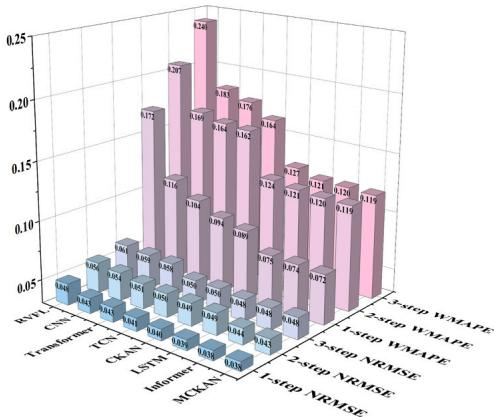
\includegraphics[keepaspectratio,alt={image}]{images/373c0cc2af00f607c3754f792466f6865b7bf6c5027e6f5c5e209b32b407e501.jpg}}

\pandocbounded{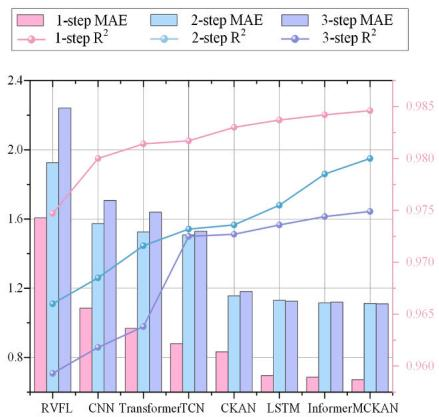
\includegraphics[keepaspectratio,alt={image}]{images/59458f7b5cf56d8df66fd3424256b4e90468df40bd5d3f94ed03c207cc52ba7e.jpg}}

\begin{enumerate}
\def\labelenumi{(\alph{enumi})}
\setcounter{enumi}{1}
\tightlist
\item
\end{enumerate}

Fig. 8. Performance comparison between MCKAN and baseline models in PV
power forecasting.

\pandocbounded{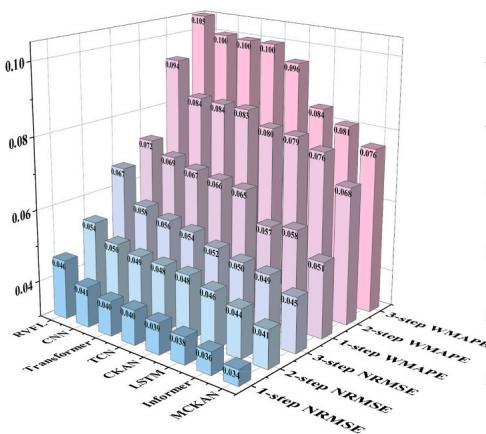
\includegraphics[keepaspectratio,alt={image}]{images/29f7e7ad64d23b00d2662ed0351a0e5595c447ac3bd593cb07defe242acaa95d.jpg}}

\pandocbounded{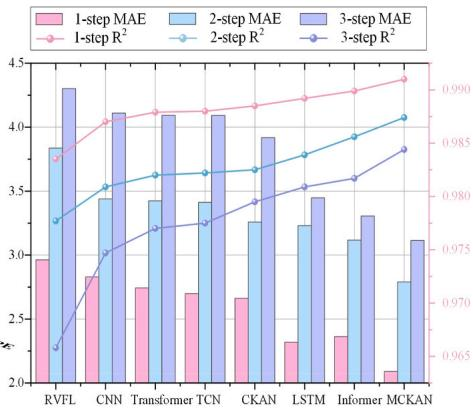
\includegraphics[keepaspectratio,alt={image}]{images/e8ea2202c990897a9d753bc7a2bd48e0bdd760b3aec78a358929e7b6731200f5.jpg}}

\begin{enumerate}
\def\labelenumi{(\alph{enumi})}
\setcounter{enumi}{1}
\tightlist
\item
\end{enumerate}

Fig. 9. Performance comparison between MCKAN and baseline models in Wind
power forecasting.

\pandocbounded{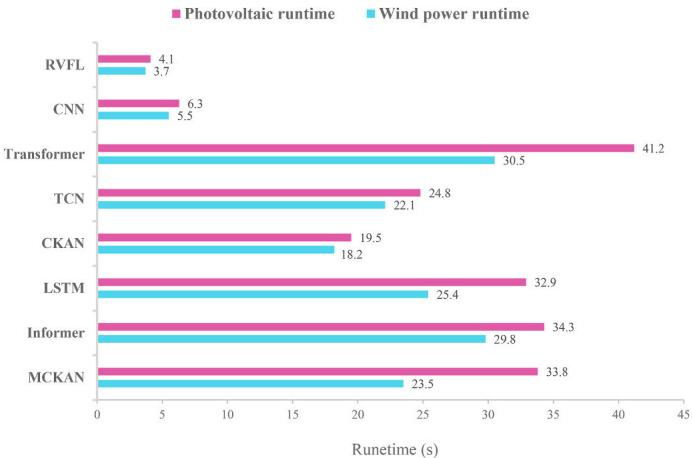
\includegraphics[keepaspectratio,alt={image}]{images/e0d012907aebab24aaa4f1e00328a7acdb95308a4c4b834956b81248ff4f501a.jpg}}

Fig. 10. Runtime analysis of baseline models.

multiple temporal scales. This capability is particularly valuable for
power grid operations, as it facilitates the management of uncertain
loads and the optimization of energy dispatch strategies. Moreover, it
contributes to improving the overall stability and controllability of
the system.

\section{5.2.2. Performance analysis with individual
components}\label{performance-analysis-with-individual-components}

To evaluate the effectiveness of each component in the proposed model,
we conduct a series of ablation experiments. These experiments are
designed to isolate and assess the impact of the attention mechanism

and the hyperparameter optimization algorithm. The overall results are
summarized in Table 4 and will be analyzed in detail in the following
sections.

In photovoltaic forecasting, the power generation has a strong
periodicity. Although the introduction of the attention mechanism does
not significantly reduce the average prediction error, it yields a
noticeable improvement in NRMSE, as shown in Fig. 11 a. Compared with
the baseline MCKAN model, the NRMSE

in 1-step forecasting is reduced by \(7 . 2 ~ \%\) with MCKAN-AT and by
\(1 5 . 6 \%\) with MCKAN-EAA. This indicates that the attention
mechanism enhances the model's ability to capture abrupt changes in
power output. Fig. 12 further supports this finding: under conditions of
power fluctuation, both MCKAN-AT (light orange) and MCKAN-EAA (light
purple) align more closely with the actual values than the basic MCKAN
model

\pandocbounded{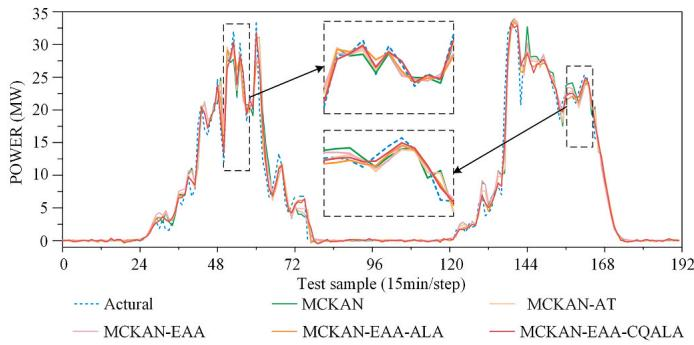
\includegraphics[keepaspectratio,alt={image}]{images/fcecb1bb4e476dee1d1b6b520261a3b2d0e0e0a06a123e3ff86ef89aa1986e4d.jpg}}

Fig. 12. Prediction curve (1 Step) of Model Variants in PV power
forecasting.

Table 4 Ablation study results of the MCKAN-EAA-CQALA model components.

{\def\LTcaptype{none} % do not increment counter
\begin{longtable}[]{@{}llllllllllll@{}}
\toprule\noalign{}
\endhead
\bottomrule\noalign{}
\endlastfoot
\multirow{2}{*}{Step} & \multirow{2}{*}{Model} & \multicolumn{5}{l}{%
Photovoltaic Power} & \multicolumn{5}{l@{}}{%
Wind Power} \\
& & WMAPE & NRMSE & MAE & R² & Runtime(s) & WMAPE & NRMSE & MAE & R² &
Runtime(s) \\
\multirow{5}{*}{1-step} & MCKAN & 0.0721 & 0.0377 & 0.6720 & 0.9846 &
33.82 & 0.0510 & 0.0344 & 2.0898 & 0.9910 & 23.53 \\
& MCKAN-AT & 0.0717 & 0.0350 & 0.6686 & 0.9867 & 39.71 & 0.0504 & 0.0338
& 2.0643 & 0.9913 & 36.44 \\
& MCKAN-EAA & 0.0715 & 0.0318 & 0.6665 & 0.9890 & 35.62 & 0.0473 &
0.0328 & 1.9368 & 0.9918 & 29.35 \\
& MCKAN-EAA-ALA & 0.0474 & 0.0210 & 0.4425 & 0.9952 & 78.51 & 0.0441 &
0.0295 & 1.8075 & 0.9934 & 67.27 \\
& MCKAN-EAA-CQALA & 0.0439 & 0.0202 & 0.4090 & 0.9956 & 72.11 & 0.0357 &
0.0244 & 1.4636 & 0.9954 & 64.91 \\
\multirow{5}{*}{2-step} & MCKAN & 0.1113 & 0.0429 & 1.0380 & 0.9800 &
36.52 & 0.0681 & 0.0406 & 2.7902 & 0.9874 & 26.11 \\
& MCKAN-AT & 0.1098 & 0.0406 & 1.0240 & 0.9821 & 43.10 & 0.0661 & 0.0394
& 2.7104 & 0.9881 & 40.30 \\
& MCKAN-EAA & 0.1089 & 0.0398 & 1.0157 & 0.9828 & 38.92 & 0.0629 &
0.0387 & 2.5797 & 0.9885 & 32.11 \\
& MCKAN-EAA-ALA & 0.0790 & 0.0383 & 0.7367 & 0.9840 & 82.71 & 0.0514 &
0.0313 & 2.1076 & 0.9925 & 72.55 \\
& MCKAN-EAA-CQALA & 0.0775 & 0.0282 & 0.7229 & 0.9913 & 77.81 & 0.0470 &
0.0292 & 1.9263 & 0.9935 & 68.10 \\
\multirow{5}{*}{3-step} & MCKAN & 0.1190 & 0.0481 & 1.1099 & 0.9749 &
37.41 & 0.0760 & 0.0452 & 3.1137 & 0.9844 & 29.50 \\
& MCKAN-AT & 0.1165 & 0.0480 & 1.0870 & 0.9750 & 46.81 & 0.0733 & 0.0426
& 3.0021 & 0.9860 & 41.73 \\
& MCKAN-EAA & 0.1159 & 0.0480 & 1.0810 & 0.9750 & 42.33 & 0.0684 &
0.0425 & 2.8027 & 0.9862 & 34.31 \\
& MCKAN-EAA-ALA & 0.1083 & 0.0457 & 1.0105 & 0.9789 & 84.22 & 0.0600 &
0.0381 & 2.4604 & 0.9889 & 75.02 \\
& MCKAN-EAA-CQALA & 0.1042 & 0.0359 & 0.9715 & 0.9860 & 77.91 & 0.0558 &
0.0360 & 2.2858 & 0.9901 & 72.61 \\
\end{longtable}
}

\pandocbounded{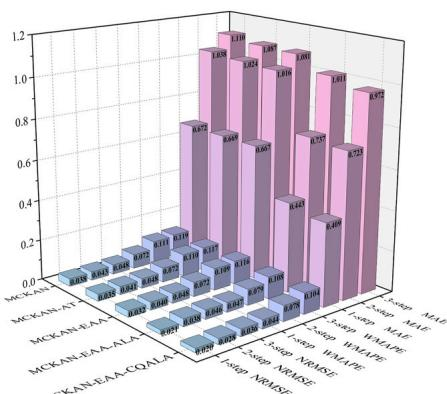
\includegraphics[keepaspectratio,alt={image}]{images/a767180d0ec4bbd045fe7c8a91dd3dae8799f079905822859c5867ceb60df3e7.jpg}}

\pandocbounded{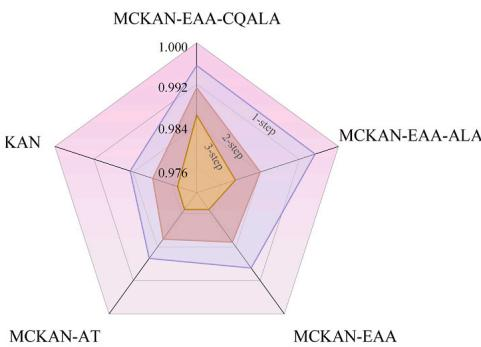
\includegraphics[keepaspectratio,alt={image}]{images/02ededa8a3b1fa31999926a214f5c6afcd02ea1f84c8214f5b545bb1c8b89d41.jpg}}

\begin{enumerate}
\def\labelenumi{(\alph{enumi})}
\setcounter{enumi}{1}
\tightlist
\item
\end{enumerate}

Fig. 11. Performance evaluation of model variants in the ablation
setting.

\pandocbounded{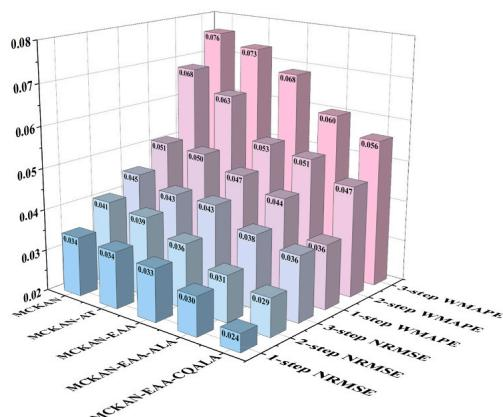
\includegraphics[keepaspectratio,alt={image}]{images/d79cdd7c1c36c7e212b81adfa526d8350f670bf2c7a1762c7c3a5258eae54891.jpg}}

\begin{enumerate}
\def\labelenumi{(\alph{enumi})}
\tightlist
\item
\end{enumerate}

\pandocbounded{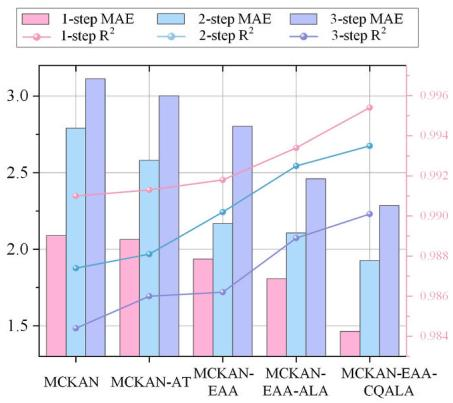
\includegraphics[keepaspectratio,alt={image}]{images/1c384082751d93f4e6cf08a9d08e163fe90858b37729fb698074b6e131e78540.jpg}}

\begin{enumerate}
\def\labelenumi{(\alph{enumi})}
\setcounter{enumi}{1}
\tightlist
\item
\end{enumerate}

Fig. 13. Performance evaluation of model variants in wind power
forecasting.

(green).

At the same time, the above results indicate that the integration of the
hyperparameter optimization algorithm significantly enhances the model's
prediction accuracy, and the prediction errors in the 1--3 step
prediction are greatly reduced. The MAE of the MCKAN-EAA-ALAS algorithm
has a maximum reduction of \(3 4 . 1 5 ~ \%\) compared with other
models, and the maximum MAE of the MCKAN-EAA-CQALA algorithm has
decreased by \(3 9 . 1 4 ~ \%\) . At the same time, the R values are
0.9956, 0.9913 and 0.986 respectively, which are more stable than other
comparison models in the 1--3 step photovoltaic prediction.

Consistent with the results observed in photovoltaic forecasting, the
integration of hyperparameter optimization also offers significant
advantages in enhancing model performance for complex wind power
prediction (see Fig. 13). Compared with the MCKAN-EAA model, the
prediction accuracy and model stability of the MCKAN-EAA-ALA model have
been greatly improved. Its WMAPE, NRMSE and MAE are reduced by
\(1 3 . 5 3 \%\) , \(1 4 . 2 4 \%\) and \(1 3 . 5 1 \ \%\) respectively
compared with the basic MCKAN in 1-step wind power forecasting, and its
NRMSE value is reduced by nearly 3 times compared with MCKAN-EAA. By
combining chaotic mapping and quasi-opposition population update
strategy to optimize the initial population generation and evolution
process of ALA, the model proposed in this paper significantly improves
the model performance while reducing the model running speed.
Specifically, it achieves WMAPE, NRMSE, and MAE values of 0.0357,
0.0244, and 1.4636, respectively, while attaining a high
\(\mathrm { R } ^ { 2 }\) value of 0.9954. Compared to the MCKAN-EAA-ALA
model, these four indicators show notable improvements of
\(1 9 . 0 5 ~ \%\) , \(1 7 . 2 9 \ \%\) , \(1 9 . 0 3 ~ \%\) , and
\(0 . 2 0 ~ \%\) , respectively.

Overall, MCKAN-EAA-CQALA shows significant performance advantages, with
the maximum improvement of WMAPE, NRMSE, MAE and
\(\mathrm { R } ^ { 2 }\) reaching \(3 0 . 0 0 \%\) , \(2 9 . 0 7 \ \%\)
, \(2 9 . 9 6 ~ \%\) and \(0 . 4 4 ~ \%\) , respectively.

\pandocbounded{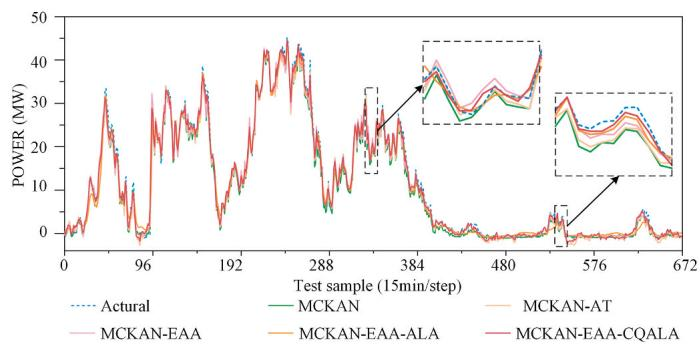
\includegraphics[keepaspectratio,alt={image}]{images/4cd16118c4fb705e6e11cf6d7dde2507e3a24ae516a1965b18fca59fa498137b.jpg}}

Fig. 14. Prediction curve (1-Step) of Model Variants in Wind power
forecasting.

These fusion experiments further demonstrate the effectiveness of the
proposed model. By introducing CQALA, the framework is able to more
accurately and dynamically adjust the hyperparameters of the hybrid
model (MCKAN-EAA), thereby enhancing its adaptability to wind and solar
energy data under complex environmental conditions and improving
prediction performance. The MCKAN-EAA-CQALA model (red) has the highest
agreement with the true value curve, both in the overall trend and at
the local peak (as shown in Fig. 14). Especially in the interval {[}520,
535{]}, the close fit at the local inflection point further confirms the
model's excellent ability to capture subtle temporal dynamics.

In ultra-short-term wind and solar forecasting, improving model accuracy
must be balanced with maintaining computational efficiency. Based on the
basic MCKAN model, the EAA attention mechanism improves the prediction
stability, especially the prediction performance under the sudden
weather changes

of the model. In the photovoltaic prediction, compared with the running
time of 33.82s of the basic model, MCKAN-EAA has a maximum NRMSE value
of \(1 5 . 6 \%\) lower when the running time is only increased by 1.8s,
which fully reflects the effectiveness of the EAA attention mechanism
for wind and solar forecasting. With the increase of the prediction
step, the prediction accuracy of the basic model continues to decrease,
and the MAE prediction value of MCKAN increases from 0.672 to 2.0898 to
1.1099 and 3.1137.

Although the application of hyperparameter optimization increases the
computational time for certain models, it significantly improves
prediction accuracy. In single-step photovoltaic forecasting, the
integration of the CQALA algorithm directly reduces the NRMSE to 0.0202.
Compared to the baseline MCKAN-EAA model, the accuracy improvement
increases significantly, with the reduction in NRMSE rising from
\(1 5 . 6 5 ~ \%\) to \(4 6 . 4 2 ~ \%\) . Meanwhile, compared to the
MCKAN-EAA-ALA algorithm, the computational time of MCKAN-EAA-CQALA is
reduced by \(8 . 1 5 ~ \%\) , with a runtime of only 72.11 s,
demonstrating excellent computational efficiency. These results confirm
the effectiveness of the chaotic and quasi-oppositional strategies in
accelerating convergence.

In multi-step forecasting, the MCKAN-EAA-CQALA model also shows a
significant improvement in prediction accuracy. In 3-step photovoltaic
forecasting, the NRMSE drops to 0.0359, which is even lower than that of
the MCKAN model in single-step prediction. In 1- to 3-step wind power
forecasting, the MAE values improve by \(3 0 . 0 \%\) , \(3 1 . 0 \%\) ,
and 26.6 \(\%\) , respectively. While the original MCKAN model reaches
an MAE of 3.1137 in 3-step forecasting, the proposed model achieves a
much lower MAE of 2.2858---only slightly higher than MCKAN's 2.0898 in
the single-step case. Additionally, in wind power forecasting scenarios,
the proposed model reduces the computational time by up to
\(6 . 1 3 \ \%\) compared to ALA.

Overall, the proposed MCKAN-EAA-CQALA model significantly

Table 5 Description of SOTA models for comparison.

{\def\LTcaptype{none} % do not increment counter
\begin{longtable}[]{@{}|l|l|l|@{}}
\toprule\noalign{}
\endhead
\bottomrule\noalign{}
\endlastfoot
\hline
Models & Component & Description \\
\hline
CNN-ABiLSTM (Bashir et al., 2025) & CNN,Attention-basedABiLSTM & CNN
captures short-term patterns in solar and wind power data.ABiLSTM learns
long-term dependencies while using attention mechanisms to focus on
critical temporal features, improving multi-horizon forecasting
accuracy. \\
\hline
COA-CNN-LSTM (Abou Houran et al., 2023) & CNN,LSTM,Coati Optimization
Algorithm (COA) & CNN and LSTM are used to extract spatial and temporal
features of wind power data. The Coati Optimization Algorithm fine-tunes
hyperparameters such as learning rate to enhance model performance,
enabling more precise short-term offshore wind forecasting. \\
\hline
NP-CNN-LSTM (Devlin et al., 2019) & Neural
Prophet,CNN,LSTM,BayesianOptimization & Neural Prophet models trends,
seasonality, and special events in load data. CNN extracts local
features, and LSTM captures long-term dependencies. Bayesian
optimization determines optimal hyperparameters, and least squares
fusion combines model outputs for improved short-term load
forecasting. \\
\hline
DWT-WaveNet-LSTM (Cui et al., 2024b) & Discrete Wavelet Transform
(DWT),WaveNet,LSTM,Attention, & DWT decomposes nonstationary
hydrological signals. WaveNet captures complex temporal dependencies,
and LSTM models long-term trends. Attention and residual connections
enhance learning of key features and prevent overfitting. A dual-branch
structure predicts discharge and residuals to refine accuracy in karst
hydrology forecasting. \\
\hline
CNN-CA-Transformer (Sanh et al., 2019) & CNN,Transformer,Cellular
Automata & Transformer quantifies heterogeneous spatial interactions via
self-attention. Local Moran\textquotesingle s I guides learning of
spatial autocorrelation. The network output, representing development
potential, is integrated into CA to simulate urban growth, improving
accuracy and interpretability in large-scale urban modeling. \\
\hline
\end{longtable}
}

enhances the forecasting accuracy and stability of the baseline MCKAN
model through the integration of EAA and CQALA, while maintaining an
effective balance between accuracy and computational efficiency. This
makes it a promising approach for intelligent forecasting in renewable
energy systems. To further verify the superiority and efficiency of the
proposed algorithm, a detailed comparison with other state-of-the-art
algorithms will be presented in the next section.

\section{5.3. Comparison with SOTA
methods}\label{comparison-with-sota-methods}

To evaluate the effectiveness of the proposed MCKAN-EAA-CQALA model,
this experiment compares it with five state-of-the-art hybrid models:
CNN-ABiLSTM(Bashir et al., 2025), COA-CNN-LSTM (Abou Houran et al.,
2023), NP-CNN-LSTM (Sanh et al., 2019), DWT-WaveNet-LSTM (Zhou et al.,
2024) and CNN-CA-Transformer (Xu et al., 2025). Table 5 provides the
composition and a brief description of each model. Based on the wind and
photovoltaic data described in the previous section, we conduct and
analyze forecasting experiments ranging from one-step to three-step
ahead. The indicators results are presented in Table 6.

In the 1-step prediction task, the MCKAN-EAA-CQALA model demonstrates
superior accuracy compared to several state-of-the-art models. For
photovoltaic power forecasting, it achieves a WMAPE of 0.0439 and an MAE
of 0.4090. Compared to the NP-CNN-LSTM model, this represents reductions
of \(2 7 . 5 6 \%\) in WMAPE and \(2 7 . 5 9 \%\) in MAE. Relative to
CNN-ABiLSTM and CNN-CA-Transformer, the MAE is reduced by 21.30 \(\%\)
and \(2 7 . 3 9 ~ \%\) , respectively. When compared to the COA-CNN-LSTM
model, the proposed approach reduces WMAPE and MAE by \(2 0 . 7 6 ~ \%\)
and \(2 0 . 7 8 ~ \%\) , respectively, while also achieving a
\(3 2 . 5 5 ~ \%\) decrease in NRMSE. Furthermore, compared with the
best-performing DWT-Wave-Net-LSTM model, the MCKAN-EAA-CQALA model
reduces WMAPE and MAE by \(1 4 . 0 6 ~ \%\) and \(1 4 . 3 1 \ \%\) ,
respectively, while maintaining shorter runtime. These results
demonstrate that MCKAN-EAA-CQALA provides more reliable and accurate
short-term photovoltaic forecasts, which are crucial for improving grid
dispatch efficiency and enhancing solar energy utilization under rapidly
changing conditions (see Fig. 14).

For wind power forecasting, the MCKAN-EAA-CQALA model achieves a WMAPE
of 0.0357 and an MAE of 1.4636, representing improvements of
\(3 3 . 5 2 \%\) and \(3 3 . 4 6 \%\) , respectively, compared to the
NP-CNN-LSTM model. Relative to CNN-ABiLSTM and CNN-CA-Transformer, the
MAE is reduced by \(2 6 . 0 0 ~ \%\) and \(2 7 . 6 4 ~ \%\) ,
respectively. When compared to COA-CNN-LSTM, the proposed model reduces
WMAPE by \(1 0 . 5 3 \%\) , NRMSE by \(2 2 . 2 9 \%\) , and MAE by
\(1 0 . 5 2 \%\) . It also outperforms the DWT-WaveNet-LSTM model, with
reductions of \(8 . 4 6 \%\)

Table 6 Performance metrics of the proposed model and SOTA models.

{\def\LTcaptype{none} % do not increment counter
\begin{longtable}[]{@{}llllllllllll@{}}
\toprule\noalign{}
\endhead
\bottomrule\noalign{}
\endlastfoot
\multirow{2}{*}{Step} & \multirow{2}{*}{Model} & \multicolumn{5}{l}{%
Photovoltaic power} & \multicolumn{5}{l@{}}{%
Wind power} \\
& & WMAPE & NRMSE & MAE & R² & Runtime(s) & WMAPE & NRMSE & MAE & R² &
Runtime(s) \\
\multirow{6}{*}{1-step} & NP-CNN-LSTM & 0.0606 & 0.0297 & 0.5649 &
0.9904 & 55.37 & 0.0537 & 0.0371 & 2.199 & 0.9894 & 37.96 \\
& CNN-CA-Transformer & 0.0604 & 0.0278 & 0.5633 & 0.9916 & 62.75 &
0.0494 & 0.0337 & 2.0226 & 0.9913 & 52.40 \\
& CNN-ABI LSTM & 0.0557 & 0.0273 & 0.5197 & 0.9919 & 59.22 & 0.0483 &
0.0309 & 1.9778 & 0.9927 & 43.13 \\
& COA-CNN-LSTM & 0.0554 & 0.0245 & 0.5163 & 0.9935 & 75.82 & 0.0399 &
0.0277 & 1.6357 & 0.9941 & 67.31 \\
& DWT-WaveNet-LSTM & 0.0512 & 0.0225 & 0.4777 & 0.9945 & 85.41 & 0.039 &
0.027 & 1.5977 & 0.9944 & 77.22 \\
& MCKAN-EAA-CQALA & 0.0439 & 0.0202 & 0.409 & 0.9956 & 72.17 & 0.0357 &
0.0244 & 1.4636 & 0.9954 & 64.92 \\
\multirow{6}{*}{2-step} & NP-CNN-LSTM & 0.092 & 0.0331 & 0.8584 & 0.9881
& 59.88 & 0.0556 & 0.0388 & 2.2802 & 0.9885 & 41.50 \\
& CNN-CA-Transformer & 0.0836 & 0.0302 & 0.7797 & 0.9901 & 67.51 &
0.0545 & 0.0359 & 2.2332 & 0.9901 & 56.81 \\
& CNN-ABI LSTM & 0.0815 & 0.0292 & 0.7603 & 0.9908 & 64.14 & 0.0507 &
0.0339 & 2.0765 & 0.9912 & 49.21 \\
& COA-CNN-LSTM & 0.0795 & 0.0286 & 0.7414 & 0.9911 & 81.96 & 0.048 &
0.033 & 1.9689 & 0.9917 & 73.65 \\
& DWT-WaveNet-LSTM & 0.079 & 0.0286 & 0.7363 & 0.9911 & 92.32 & 0.0478 &
0.0326 & 1.957 & 0.9919 & 84.52 \\
& MCKAN-EAA-CQALA & 0.0775 & 0.0282 & 0.7229 & 0.9913 & 74.81 & 0.047 &
0.0292 & 1.9263 & 0.9935 & 68.11 \\
\multirow{6}{*}{3-step} & NP-CNN-LSTM & 0.1208 & 0.0442 & 1.1265 &
0.9788 & 64.20 & 0.06 & 0.0413 & 2.4595 & 0.987 & 45.22 \\
& CNN-CA-Transformer & 0.1175 & 0.0421 & 1.0957 & 0.9808 & 72.11 &
0.0578 & 0.039 & 2.3673 & 0.9884 & 61.87 \\
& CNN-ABI LSTM & 0.1111 & 0.042 & 1.036 & 0.9812 & 70.31 & 0.0577 &
0.0379 & 2.3652 & 0.989 & 53.82 \\
& COA-CNN-LSTM & 0.1074 & 0.0414 & 1.002 & 0.9814 & 85.70 & 0.0575 &
0.0369 & 2.3563 & 0.9896 & 78.95 \\
& DWT-WaveNet-LSTM & 0.1062 & 0.0396 & 0.9904 & 0.9831 & 97.63 & 0.0568
& 0.0365 & 2.3273 & 0.9897 & 90.22 \\
& MCKAN-EAA-CQALA & 0.1042 & 0.0359 & 0.9715 & 0.986 & 77.92 & 0.0558 &
0.036 & 2.2858 & 0.9901 & 72.60 \\
\end{longtable}
}

\pandocbounded{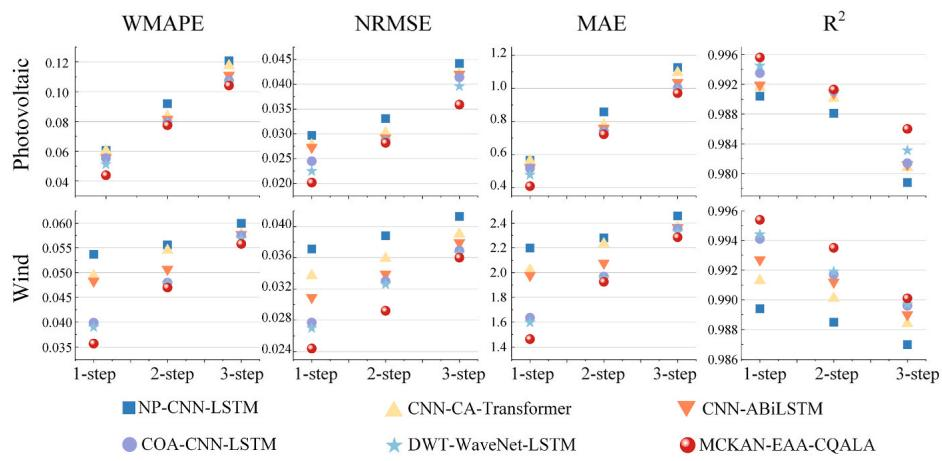
\includegraphics[keepaspectratio,alt={image}]{images/05e56e30f72d7b65a6ba19bc3a67fecf19ac2d4d950a41b7d20f0d9179d85204.jpg}}

Fig. 15. Comparison of evaluation metrics between the proposed model and
SOTA methods.

\pandocbounded{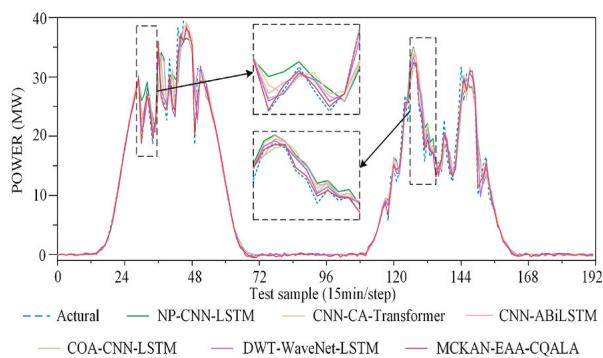
\includegraphics[keepaspectratio,alt={image}]{images/6d1c4db61c13bee697bc431843d0d787faf289a0b9c932104a3d81bb7188dfc9.jpg}}

a）1-Step PV power forecasting

\pandocbounded{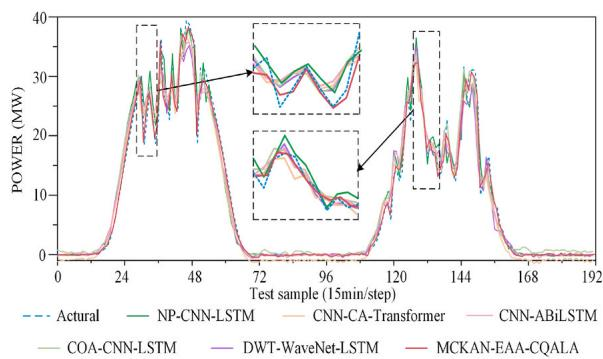
\includegraphics[keepaspectratio,alt={image}]{images/9e5816c6d1f2c4772efcdb7c1a08ef79ad5462c55cc9fb41cc91cfcc220f9ff0.jpg}}

\begin{enumerate}
\def\labelenumi{\alph{enumi})}
\setcounter{enumi}{2}
\tightlist
\item
  2-Step PV power forecasting
\end{enumerate}

\pandocbounded{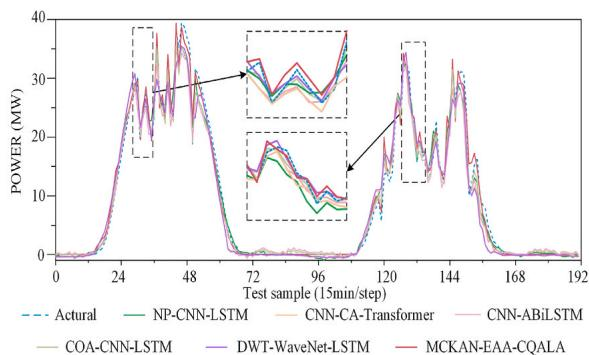
\includegraphics[keepaspectratio,alt={image}]{images/5a52fced27efb6e357d63bffd898183c94a24ead7658508f61d4950c1d2597c9.jpg}}

\begin{enumerate}
\def\labelenumi{\alph{enumi})}
\setcounter{enumi}{4}
\tightlist
\item
  3-Step PV power forecasting
\end{enumerate}

\pandocbounded{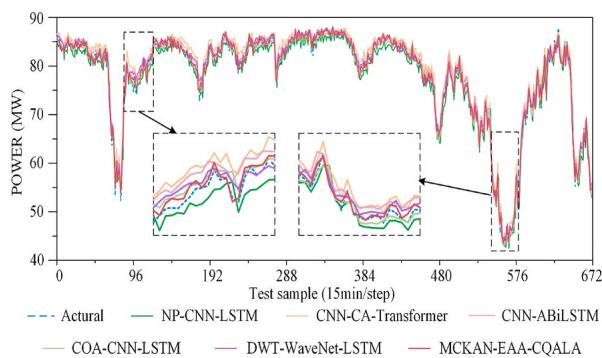
\includegraphics[keepaspectratio,alt={image}]{images/0b9557d08a7bebce68b2e1d88a0361513a1279045bb7e5cc456c06e89fc8a8ca.jpg}}

\begin{enumerate}
\def\labelenumi{\alph{enumi})}
\setcounter{enumi}{1}
\tightlist
\item
  1-Step Wind power forecasting
\end{enumerate}

\pandocbounded{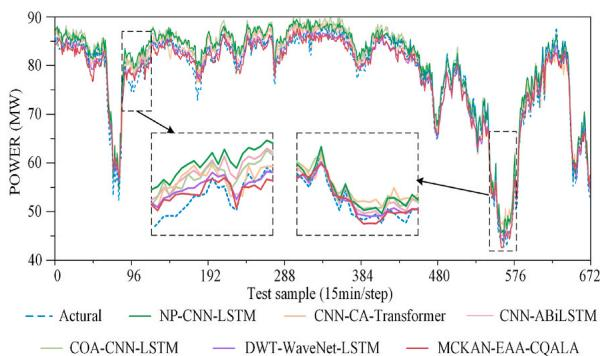
\includegraphics[keepaspectratio,alt={image}]{images/d129d342d135d05e5196f08e642e740e0282006ec678367d080bc4ae46570524.jpg}}

\begin{enumerate}
\def\labelenumi{\alph{enumi})}
\setcounter{enumi}{3}
\tightlist
\item
  2-Step Wind power forecasting
\end{enumerate}

\pandocbounded{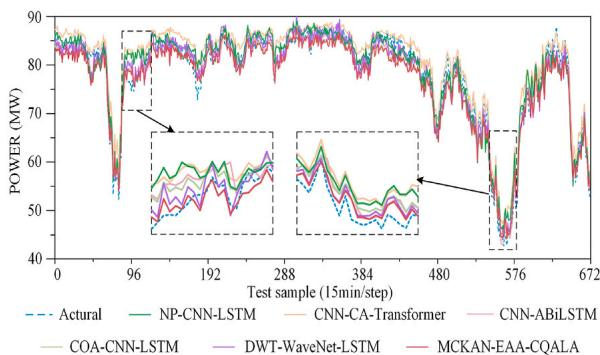
\includegraphics[keepaspectratio,alt={image}]{images/10a40c54aa013d94bf2567010412cf44bf6a386cca4788d1f442c76b378d534d.jpg}}

\begin{enumerate}
\def\labelenumi{\alph{enumi})}
\setcounter{enumi}{5}
\tightlist
\item
  3-Step Wind power forecasting
\end{enumerate}

Fig. 16. Prediction curves comparing the proposed model and SOTA methods
over 1--3 steps.

in WMAPE, \(8 . 4 0 ~ \%\) in MAE, and \(1 5 . 9 3 \ \%\) in computation
time. As visualized in Fig. 15, the proposed model consistently
outperforms other SOTA methods across all evaluation metrics. These
results highlight the effectiveness of the model's robust multi-scale
feature extraction capability, enabled by the parallel structure of
MCKAN, and its efficient noise reduction mechanism (EAA), which

assigns greater weight to key predictive features while suppressing
irrelevant information. In addition, the CQALA algorithm contributes to
enhanced training stability and convergence speed, enabling superior
short-term forecasting accuracy for both photovoltaic and wind power
datasets.

In the multi-step forecasting task, the MCKAN-EAA-CQALA model maintains
strong predictive performance across both PV and wind power scenarios.
For PV forecasting, the model achieves WMAPE values of 0.0775 and 0.1042
in 2-step and 3-step predictions, respectively, representing
improvements of \(1 5 . 7 6 ~ \%\) and \(1 3 . 7 4 \ \%\) over
NP-CNN-LSTM. Compared to other strong baselines, MCKAN-EAA-CQALA
consistently outperforms CNN-CA-Transformer, CNN-ABiLSTM, COA-CNN-LSTM,
and DWT-WaveNet-LSTM. For instance, in 3-step PV forecasting, it
achieves a \(9 . 3 6 \%\) reduction in MAE and a \(1 . 9 0 \%\)
reduction in NRMSE compared to DWT-WaveNet-LSTM, which is among the most
competitive SOTA models. These results highlight the model's robustness
in maintaining accuracy over longer forecasting horizons, which is
essential for day-ahead solar dispatching and planning.

In wind power forecasting, the model also demonstrates notable accuracy
despite the increased uncertainty and nonlinearity inherent in wind
generation. It achieves MAEs of 1.9263 and 2.2858 in 2-step and 3- step
predictions, yielding reductions of \(1 5 . 5 2 \%\) and \(7 . 0 6 \%\)
compared to NP-CNN-LSTM. Compared to CNN-ABiLSTM and CNN-CA-Transformer,
the proposed model achieves \(1 3 . 8 4 \ \%\) and \(3 . 4 4 \ \%\)
lower MAEs, respectively, in 3-step forecasting. Even against strong
models like COA-CNN-LSTM and DWT-

WaveNet-LSTM, the proposed method maintains a clear advantage.
Specifically, in 2-step prediction, it reduces MAE by \(3 . 6 4 \%\) and
\(4 . 1 5 \%\) , respectively, and further narrows the error gap in
3-step forecasting. The proposed model demonstrates favorable
performance in multi-step forecasting for both wind and solar energy,
while maintaining relatively low computational cost. These findings
illustrate that MCKAN-EAA-CQALA is capable of effectively capturing
short-term fluctuations

and maintaining long-term predictive stability, achieving generally
competitive results compared to a wide range of advanced SOTA baselines
across both energy domains.

Fig. 16 presents the visualization of forecasting results. As the
forecasting horizon extends, the prediction task becomes more
challenging, leading to increasing deviations between the model outputs
and actual values. This trend is especially pronounced during periods of
significant weather variability, such as time intervals (Zhu et al.,
2021; Nguyen-Duc et al., 2024) in the PV data and {[}96, 160{]} in the
wind power data. In the PV forecasting task, NP-CNN-LSTM (green) and
CNN-CA-Transformer (orange) exhibit poor stability and significant
deviations in multi-step predictions. Although other baseline models
maintain relatively low forecasting errors, they fail to capture rapid
trend changes, particularly within the 26--36 interval of the three-step
prediction. Only MCKAN-EAA-CQALA (red) consistently tracks the actual
trends across the entire forecasting period.

In multi-step wind power forecasting, the MCKAN-EAA-CQALA model
consistently outperforms baseline models such as NP-CNN-LSTM,
CNN-CA-Transformer, and COA-CNN-LSTM in terms of both stability and
trend-fitting performance across single-step and multi-step scenarios.
To further assess the robustness of the proposed model under extreme
weather conditions, the following section analyzes its performance
during summer and winter events.

\section{5.4. Discussion of model performance under extreme weather
conditions}\label{discussion-of-model-performance-under-extreme-weather-conditions}

Forecasting models are often sensitive to drastic seasonal variations,
which may result in unstable performance under extreme climate
conditions. To further evaluate the model's performance under extreme
weather conditions, this study analyzes its behavior during periods of
significant seasonal variation. In the North China region, the summer
season is marked by high cloud cover, intense precipitation, and
elevated humidity, all of which substantially increase the variability
of solar irradiance. Moreover, strong convective activity induces abrupt
changes in wind fields and intensifies turbulence, further amplifying
the intermittency of wind power output. In contrast, winter is dominated
by stable cold high-pressure systems, resulting in clear skies and
minimal cloud cover. Under these conditions, solar irradiance becomes
highly predictable, and prevailing winds remain steady with relatively
weak

Table 7 Seasonal performance comparison of the proposed model and SOTA
models.

{\def\LTcaptype{none} % do not increment counter
\begin{longtable}[]{@{}lllllllllll@{}}
\toprule\noalign{}
\endhead
\bottomrule\noalign{}
\endlastfoot
\multirow{2}{*}{Season} & \multirow{2}{*}{Step} & \multirow{2}{*}{Model}
& \multicolumn{4}{l}{%
Photovoltaic} & \multicolumn{4}{l@{}}{%
Wind power} \\
& & & WMAPE & NRMSE & MAE & R² & WMAPE & NRMSE & MAE & R² \\
\multirow{12}{*}{Summer} & \multirow{6}{*}{1-step} & NP-CNN-LSTM &
0.0763 & 0.0408 & 0.7806 & 0.9831 & 0.1406 & 0.0491 & 2.2983 & 0.9532 \\
& & CNN-CA-Transformer & 0.0716 & 0.0369 & 0.7331 & 0.9862 & 0.1178 &
0.0414 & 1.9253 & 0.9667 \\
& & CNN-ABiLSTM & 0.0702 & 0.0354 & 0.7191 & 0.9873 & 0.1103 & 0.0389 &
1.8028 & 0.9706 \\
& & COA-CNN-LSTM & 0.0664 & 0.0344 & 0.6804 & 0.988 & 0.1041 & 0.037 &
1.702 & 0.9734 \\
& & DWT-WaveNet-LSTM & 0.0614 & 0.0316 & 0.6288 & 0.9899 & 0.0968 &
0.034 & 1.5830 & 0.9776 \\
& & MCKAN-EAA-CQALA & 0.0556 & 0.0290 & 0.5699 & 0.9915 & 0.0900 &
0.0312 & 1.4714 & 0.9811 \\
& \multirow{6}{*}{3-step} & NP-CNN-LSTM & 0.1348 & 0.0556 & 1.382 &
0.9687 & 0.1363 & 0.0462 & 2.2288 & 0.9585 \\
& & CNN-CA-Transformer & 0.1296 & 0.0526 & 1.3289 & 0.972 & 0.1287 &
0.0431 & 2.1045 & 0.9639 \\
& & CNN-ABiLSTM & 0.1274 & 0.0514 & 1.306 & 0.9733 & 0.1249 & 0.0427 &
2.0427 & 0.9647 \\
& & COA-CNN-LSTM & 0.1248 & 0.0509 & 1.2792 & 0.9738 & 0.1344 & 0.0419 &
2.1981 & 0.9657 \\
& & DWT-WaveNet-LSTM & 0.1209 & 0.0497 & 1.2391 & 0.9751 & 0.1323 &
0.0407 & 2.1634 & 0.9678 \\
& & MCKAN-EAA-CQALA & 0.1127 & 0.0468 & 1.1548 & 0.9778 & 0.1318 &
0.0394 & 2.1551 & 0.9699 \\
\multirow{12}{*}{Winter} & \multirow{6}{*}{1-step} & NP-CNN-LSTM &
0.0537 & 0.024 & 0.4345 & 0.9943 & 0.0471 & 0.0428 & 2.672 & 0.9813 \\
& & CNN-CA-Transformer & 0.0502 & 0.0236 & 0.4084 & 0.9937 & 0.0422 &
0.038 & 2.3966 & 0.9853 \\
& & CNN-ABiLSTM & 0.0494 & 0.0221 & 0.3998 & 0.9952 & 0.041 & 0.0342 &
2.3268 & 0.9881 \\
& & COA-CNN-LSTM & 0.0487 & 0.0212 & 0.3947 & 0.9956 & 0.0346 & 0.0315 &
1.9635 & 0.9899 \\
& & DWT-WaveNet-LSTM & 0.0468 & 0.0194 & 0.3793 & 0.9963 & 0.0344 &
0.0312 & 1.9527 & 0.9901 \\
& & MCKAN-EAA-CQALA & 0.0418 & 0.0173 & 0.3379 & 0.9970 & 0.0307 & 0.028
& 1.7415 & 0.992 \\
& \multirow{6}{*}{3-step} & NP-CNN-LSTM & 0.1241 & 0.0373 & 1.0031 &
0.9862 & 0.0552 & 0.0501 & 3.1317 & 0.9744 \\
& & CNN-CA-Transformer & 0.1201 & 0.0353 & 0.97 & 0.9877 & 0.0551 &
0.0487 & 3.1297 & 0.9759 \\
& & CNN-ABiLSTM & 0.1158 & 0.0399 & 0.9354 & 0.9843 & 0.0535 & 0.0454 &
3.0350 & 0.9790 \\
& & COA-CNN-LSTM & 0.1029 & 0.0359 & 0.8318 & 0.9873 & 0.0513 & 0.0434 &
2.9121 & 0.9808 \\
& & DWT-WaveNet-LSTM & 0.1016 & 0.0338 & 0.8209 & 0.9887 & 0.051 &
0.0424 & 2.8947 & 0.9817 \\
& & MCKAN-EAA-CQALA & 0.0961 & 0.0328 & 0.7765 & 0.9894 & 0.0502 &
0.0401 & 2.8488 & 0.9837 \\
\end{longtable}
}

turbulence, leading to a more consistent pattern of wind power
generation.

The model performance indicators for summer and winter are presented in
Table 7. For photovoltaic data, prediction performance in summer
declined compared with the annual average, with NRMSE.

increasing by
\(2 2 . 3 8 \ { } ^ { 0 } / { } _ { 0 - } 3 0 . 3 6 \ { } ^ { 0 } / { } _ { 0 }\)
and \(\mathrm { R } ^ { 2 }\) decreasing by
\(0 . 7 7 \ \% { - 1 . 0 3 }\) \(\%\) ; while the prediction error in
winter has decreased, with the corresponding indicators decreasing by
\(5 . 0 0 \% - 1 6 . 1 5 \%\) and \(\mathtt { R } ^ { 2 }\) increasing
by \(0 . 3 2 \ \% - 0 . 7 6 \ \%\) . For wind power data, summer
prediction accuracy also declined relative to the annual average, with
NRMSE increasing by 9.44 \(\% - 1 3 . 5 5 ~ \%\) and
\(\mathrm { R } ^ { 2 }\) decreasing by
\(2 . 0 4 ~ \% { - 2 . 8 9 } ~ \%\) . Conversely, winter performance
improved significantly, with error metrics decreasing by
\(1 1 . 3 9 \ { \% } - 2 4 . 8 7 \ { \% }\) and
\(\mathrm { R } ^ { 2 }\) increasing

by \(0 . 6 5 ~ \% - 1 . 2 8 ~ \%\) . These results highlight the dual
impact of North China's temperate monsoon climate on renewable energy
forecasting. In summer, high precipitation, dense cloud cover, and
humidity cause large fluctuations in solar irradiance and reduce wind
speed stability, thereby limiting the forecasting accuracy for both
photovoltaic and wind power. In contrast, the winter climate is
dominated by strong cold air and the Siberian high-pressure system,
resulting in high and stable wind speeds. In addition, the stable
atmosphere and consistent irradiance enhance the predictability of
photovoltaic output.

Although seasonal variation significantly affects photovoltaic power
data, MCKAN-EAA-CQALA consistently maintains high prediction accuracy.
Compared to other state-of-the-art models, the proposed method reduces
the NRMSE of photovoltaic data by values ranging from \(5 . 8 4 \%\) to
\(1 5 . 8 3 \%\) in summer and from \(2 . 9 6 \%\) to \(1 7 . 7 9 \%\)
in winter. For wind power data, the NRMSE is reduced by
\(3 . 1 9 \ \% - 1 4 . 7 2 \ \%\) in summer and
\(5 . 4 2 \ \% - 1 9 . 9 6 \ \%\) in winter. These results demonstrate
that the proposed model exhibits strong adaptability to non-stationary
data and holds significant potential for accurate photovoltaic
forecasting under conditions of rapid climate change.

Fig. 17 provides an intuitive comparison of photovoltaic power output
between summer and winter. In summer, power generation is higher and
exhibits larger fluctuations, whereas in winter, it is lower, with
smaller and more gradual variations. Furthermore, during periods of
intense fluctuation in photovoltaic or wind power generation, the
MCKAN-EAA-CQALA model (red) closely matches the actual power

output (blue), demonstrating superior fitting performance. This
highlights the model's practical significance in enhancing the
reliability of wind and solar forecasting systems and supporting the
stable operation of power grids with high levels of renewable energy
integration.

These results highlight the significant influence of North China's
temperate monsoon climate on renewable energy forecasting accuracy and,
consequently, on grid stability. In summer, increased precipitation,
dense cloud cover, and high humidity introduce large fluctuations in
solar irradiance and reduce wind speed stability, leading to notable
declines in forecasting accuracy for both photovoltaic and wind power.
Such reduced accuracy increases operational uncertainty, requiring
higher levels of spinning reserves and resulting in greater risks of
curtailment, especially during peak load periods. In contrast, the
winter season is characterized by strong and stable winds driven by the
Siberian high-pressure system, along with clearer atmospheric conditions
that enhance the predictability of both solar and wind outputs. This
seasonal contrast emphasizes that forecasting accuracy is not only a
technical metric but also a key factor in ensuring reliable and
economical grid operation. Improving forecast precision in challenging
periods like summer is therefore essential for reducing reserve costs,
minimizing curtailment rates, and supporting the efficient integration
of renewable energy into the power system, which ultimately contributes
to greater \(\mathrm { C O } _ { 2 }\) emission reductions through more
effective utilization of clean energy.

\section{6. Conclusion}\label{conclusion}

To address the challenges posed by the intermittency and volatility of
wind and solar energy in large-scale power integration, this paper
proposes an advanced deep learning-based -based forecasting framework,
MCKAN-EAA-CQALA, for multi-step prediction of photovoltaic and wind
power outputs. The proposed multi-dimensional convolutional neural
network, MCKAN, effectively addresses the limitations of traditional
statistical approaches and shallow learning models. Through a parallel
multi-scale convolutional architecture, it captures diverse
spatiotemporal features while preserving a compact and computationally
efficient structure. This design facilitates more accurate modeling of
complex patterns inherent in renewable energy data. Simultaneously,

\pandocbounded{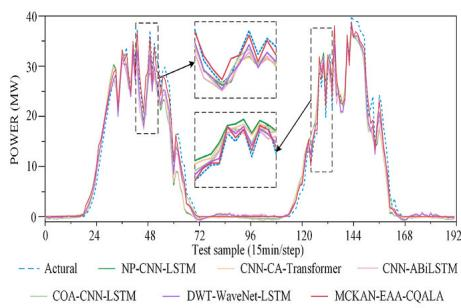
\includegraphics[keepaspectratio,alt={image}]{images/b8226e654427a4ef2913e1d695a9a8808521d86beb261126c3e01bde402a5b98.jpg}}

a)3-Step PV Power Forecasting in Summer

\pandocbounded{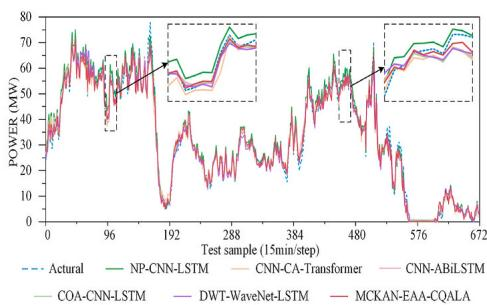
\includegraphics[keepaspectratio,alt={image}]{images/0f5e533395325155efd95cee7b2a190bc358b9aa80c944d11fcbb13fe238c745.jpg}}

\begin{enumerate}
\def\labelenumi{\alph{enumi})}
\setcounter{enumi}{1}
\tightlist
\item
  3-Step Wind Power forecasting in Summer
\end{enumerate}

\pandocbounded{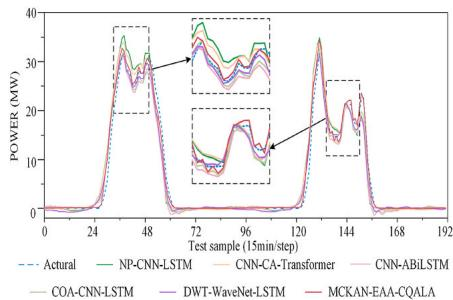
\includegraphics[keepaspectratio,alt={image}]{images/d3f1389f86701ac72593b5444d2c12fa6d8b30adfa9bbece3ebd272447a87097.jpg}}

c )3-Step PV Power forecasting in Winter

\pandocbounded{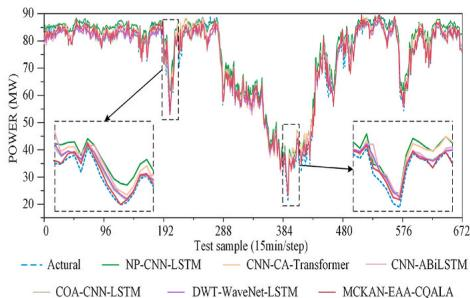
\includegraphics[keepaspectratio,alt={image}]{images/d5666c8b480f885c8791f407a864ea56065a6c74f34ad41e2941e06039b6c360.jpg}}

\begin{enumerate}
\def\labelenumi{\alph{enumi})}
\setcounter{enumi}{3}
\tightlist
\item
  3-Step Wind Power forecasting in Winter
\end{enumerate}

Fig. 17. Comparison of the prediction curves of the proposed model and
SOTA methods in summer and winter.

the Efficient Additive Attention (EAA) mechanism enhances the model's
focus on critical channel features and long-range dependencies, thereby
improving its performance in sequential and temporal modeling.
Additionally, the improved Chaotic Quasi-Ant Lemming Algorithm CQALA
integrates a chaotic quasi-reverse strategy to improve population
initialization. This approach reduces sensitivity to initial population
parameters, which is essential for maintaining prediction accuracy and
model stability.

To evaluate the effectiveness of the proposed model in multi-step
forecasting, comprehensive experiments were conducted using a twoyear
wind and solar power dataset with 15-min resolution. The model was
benchmarked against five state-of-the-art approaches: NP-CNN-LSTM,
CNN-CA-Transformer, CNN-ABiLSTM, COA-CNN-LSTM, and DWT-WaveNet-LSTM.
Experimental results demonstrate that the proposed framework
consistently outperforms both baseline and advanced models across
multiple error metrics. Specifically, it achieves reductions in MAE and
WMAPE ranging from \(1 . 7 8 \%\) to \(3 3 . 4 4 \%\) and
\(1 . 8 8 \% - 3 3 . 5 2\) \(\%\) , respectively. Under the extreme
weather conditions, the proposed model still outcomes the SOTA methods,
it reduces the NRMSE of photovoltaic forecasting by
\(5 . 8 4 \ \% - 1 5 . 8 3 \ \%\) in summer and \(2 . 9 6 ~ \%\)
\(1 7 . 7 9 \ \%\) in winter, while for wind power forecasting, NRMSE
improvements range from \(3 . 1 9 \%\) to \(1 4 . 7 2 \%\) in summer and
\(5 . 4 2 \% - 1 9 . 9 6\) \(\%\) in winter. These results highlight the
model's superior accuracy and robustness under varying seasonal and
resource conditions.

Experimental results demonstrate the model's strong performance in
ultra-short-term forecasting. The integration of AI-based methods
significantly improves prediction accuracy, enabling efficient and
lowcarbon renewable energy scheduling. While the model achieves
promising results under most conditions, its performance under climate
variability remains a challenge.

Future research will incorporate the physical characteristics of
photovoltaic and wind turbines to develop Physics-Informed Neural
Network (PINN) models for further accuracy enhancement. In addition, by
integrating AI-driven weather forecasting and federated learning, the
model will be extended to medium- and long-term forecasting and deployed
across large-scale power station networks, thereby improving grid
reliability, operational planning, and real-time management.

\section{CRediT authorship contribution
statement}\label{credit-authorship-contribution-statement}

Siyuan Chen: Writing -- original draft, Software. Hang Wan: Writing --
original draft, Methodology, Conceptualization. Botao Peng: Validation,
Software. Rui Quan: Methodology, Data curation. Yufang Chang: Writing --
review \& editing, Project administration. William Derigent: Writing --
review \& editing.

\section{Declarations}\label{declarations}

Conflicts of interest Authors declare that they do not have any
conflicts of interest.

\section{Declaration of competing
interest}\label{declaration-of-competing-interest}

The authors declare that they have no known competing financial
interests or personal relationships that could have appeared to
influence the work reported in this paper.

\section{Acknowledgment}\label{acknowledgment}

This paper was supported by the National Natural Science Foundation of
China (Grant No.~62473133), the Natural Science Foundation of Hubei
Province (Grant No.~2024AFB831) and the Natural Science Foundation of
Wuhan (Grant No.~2025040601020155).

\section{Data availability}\label{data-availability}

Data will be made available on request.

\section{References}\label{references}

Abdel-Nasser, M., Mahmoud, K., 2019. Accurate photovoltaic power
forecasting models using deep LSTM-RNN. Neural Comput. Appl. 31 (7),
2727--2740.

Abou Houran, M., Bukhari, S.M.S., Zafar, M.H., et al., 2023.
COA-CNN-LSTM: coati optimization algorithm-based hybrid deep learning
model for PV/wind power forecasting in smart grid applications. Appl.
Energy 349, 121638.

Almeida, M.P., Munoz, ˜ M., de la Parra, I., Perpin˜an, ´ O., 2017.
Comparative study of PV power forecast using parametric and
nonparametric PV models. Sol. Energy 155, 854--866.

Aslam, S., Herodotou, H., Mohsin, S.M., et al., 2021. A survey on deep
learning methods for power load and renewable energy forecasting in
smart microgrids. Renew. Sustain. Energy Rev.~144, 110992.

Bashir, T., Wang, H., Tahir, M., et al., 2025. Wind and solar power
forecasting based on hybrid CNN-ABiLSTM, CNN-transformer-MLP models.
Renew. Energy 239, 122055.

Bischl, B., Binder, M., Lang, M., et al., 2023. Hyperparameter
optimization: foundations, algorithms, best practices, and open
challenges. Wiley Interdiscipl. Rev.: Data Min. Knowl. Discov. 13 (2),
e1484.

Bodner, A.D., Tepsich, A.S., Spolski, J.N., et al., 2024. Convolutional
Kolmogorov-Arnold networks. arXiv preprint arXiv:2406.13155.

Buhan, S., Ozkazanç, ¨ Y., Çadırcı, I., 2016. Wind pattern recognition
and reference wind mast data correlations with NWP for improved
wind-electric power forecasts. IEEE Trans. Ind. Inf. 12 (3), 991--1004.

Chen, Y., Xu, J., 2022. Solar and wind power data from the Chinese state
grid renewable energy generation forecasting competition. Sci. Data 9
(1), 577.

Chung, W.H., Gu, Y.H., Yoo, S.J., 2022. District heater load forecasting
based on machine learning and parallel CNN-LSTM attention. Energy 246,
123350.

Cui, X., Zhang, X., Niu, D., 2024a. A new framework for ultra-short-term
electricity load forecasting model using IVMD--SGMD two--layer
decomposition and INGO--BiLSTM--TPA--TCN. Appl. Soft Comput. 167,
112311.

Cui, S., Lyu, S., Ma, Y., Wang, K., 2024b. Improved informer PV power
short-term prediction model based on weather typing and AHA-VMD-MPE.
Energy 307, 132766.

Cui, J., Zhang, Y., Chen, H., et al., 2025. CSWin-MBConv: a dual-network
fusing CNN and transformer for weed recognition. Eur. J. Agron. 164,
127528.

Devaraj, J., Madurai Elavarasan, R., Shafiullah, G.M., et al., 2021. A
holistic review on energy forecasting using big data and deep learning
models. Int. J. Energy Res. 45 (9), 13489--13530.

Devlin, J., Chang, M.-W., Lee, K., et al., 2019. BERT: pre-training of
deep bidirectional transformers for language understanding. In:
Proceedings of NAACL-HLT 2019, pp.~4171--4186.

Dolara, A., Leva, S., Manzolini, G., 2015. Comparison of different
physical models for PV power output prediction. Sol. Energy 119, 83--99.

ElRobrini, F.M., Bukhari, S.M.S., Zafar, M.H., et al., 2024. Federated
learning and nonfederated learning based power forecasting of
photovoltaic/wind power energy systems: a systematic review. Energy AI
18, 100438.

He, L., Liu, Y.L., Tang, Z.J., et al., 2025. Intensified excessive
wastage of key raw metals with expansion of global wind and solar
photovoltaic energy development. Resour. Conserv. Recycl. 215, 108127.

Hou, J., Su, T., Gao, T., et al., 2025. Early prediction of battery
lifetime for lithium-ion batteries based on a hybrid clustered CNN
model. Energy 319, 134992.

Hu, B., Li, W., Lu, W., et al., 2025. Integrating InSAR data and
LE-Transformer for foundation pit deformation prediction. Remote Sens.
17 (6), 1106.

Ibrahim, H., 2023. Energy management strategies of hybrid renewable
energy systems. Renew. Sustain. Energy Rev.~182, 113362.

International Energy Agency, 2024. Renewables 2024. Retrieved from.
https://www.iea. org/reports/renewables-2024.

Jin, Z., Fu, X., Xiang, L., et al., 2025. Informer learning framework
based on secondary decomposition for multi-step forecast of ultra-short
term wind speed. Eng. Appl. Artif. Intell. 139, 109702.

Jonathan, A.L., Cai, D., Ukwuoma, C.C., et al., 2024. A radiant shift:
attention-embedded CNNs for accurate solar irradiance forecasting and
prediction from sky images. Renew. Energy 234, 121133.

Kruitwagen, L., Story, K.T., Friedrich, J., et al., 2021. A global
inventory of photovoltaic solar energy generating units. Nature 598
(7882), 604--610.

Kundu, T., Garg, H., 2025. An adaptive neural network algorithm with
quasi oppositionbased learning for numerical optimization problems.
Cognitive Computation 17 (1), 55.

Li, Q., Bai, Y., Gao, W., 2021. Improved initialization method for
metaheuristic algorithms: a novel search space view. IEEE Access 9,
121366--121384.

Li, C., Shah, N., Li, \(Z _ { * , }\) et al., 2024a. Modelling of wind
and solar power output uncertainty in power systems based on historical
data: a characterisation through deterministic parameters. J. Clean.
Prod. 484, 144233.

Li, P., Yang, H., Wu, H., et al., 2024b. Deep learning model for solar
and wind energy forecasting considering Northwest China as an example.
Results Eng. 24, 102939.

Li, Q., Wang, G., Wu, X., et al., 2024c. Arctic short-term wind speed
forecasting based on CNN-LSTM model with CEEMDAN. Energy 299, 131448.

Limouni, T., Yaagoubi, R., Bouziane, K., et al., 2023. Accurate one step
and multistep forecasting of very short-term PV power using LSTM-TCN
model. Renew. Energy 205, 1010--1024.

Lindig, S., Kaaya, I., Weiß, K.A., et al., 2018. Review of statistical
and analytical degradation models for photovoltaic modules and systems
as well as related improvements. IEEE J. Photovoltaics 8 (6),
1773--1786.

Liu, X., 2025. Proposing an innovative model for solar irradiance and
wind speed forecasting. Appl. Therm. Eng. 262, 125224.

Liu, W., Mao, Z., 2024. Short-term photovoltaic power forecasting with
feature extraction and attention mechanisms. Renew. Energy 226, 120437.

Liu, J., Yan, J., Wang, L., et al., 2021. Remote sensing time series
classification based on self-attention mechanism and time sequence
enhancement. Remote Sens. 13 (9), 1804.

Liu, Z., Wang, Y., Vaidya, S., et al., 2024. Kan: Kolmogorov-arnold
networks. arXiv preprint arXiv:2404.19756.

Malhotra, R., Addis, M.T., 2024. Handwritten Amharic word recognition
with additive attention mechanism. IEEE Access.

Moreno, S.R., Seman, L.O., Stefenon, S.F., et al., 2024. Enhancing wind
speed forecasting through synergy of machine learning, singular spectral
analysis, and variational mode decomposition. Energy 292, 130493.

Mubarak, A.S., Ameen, Z.S., Mati, S., et al., 2024. Quasi-Newton
optimised Kolmogorov--Arnold Networks for wind farm power prediction.
Heliyon 10 (23), e40799.

Nguyen-Duc, T., Do-Dinh, H., Fujita, G., et al., 2024. Multi
2D-CNN-based model for short-term PV power forecast embedded with
Laplacian attention. Energy Rep.~12, 2086--2096.

Qi, Y., Jiang, A., Gao, Y., 2024. A Gaussian convolutional optimization
algorithm with tent chaotic mapping. Sci. Rep.~14 (1), 3102.

Quan, R., Zhang, J., Li, X., et al., 2024a. A hybrid CNN--BiLSTM--AT
model optimized with enhanced whale optimization algorithm for remaining
useful life forecasting of fuel cell. AIP Adv. 14 (2).

Quan, R., Qiu, Z., Wan, H., et al., 2024b. Dung beetle optimization
algorithm-based hybrid deep learning model for ultra-short-term PV power
prediction. iScience 27 (11).

Raza, M.A., Karim, A., Aman, M.M., et al., 2025. Global progress towards
the coal: tracking coal reserves, coal prices, electricity from coal,
carbon emissions and coal phase-out. Gondwana Res. 139, 43--72.

Ren, X., Zhang, F., Zhu, H., et al., 2022. Quad-kernel deep
convolutional neural network for intra-hour photovoltaic power
forecasting. Appl. Energy 323, 119682.

Ren, X., Zhang, F., Yan, J., et al., 2024. A novel convolutional neural
net architecture based on incorporating meteorological variable inputs
into ultra-short-term photovoltaic power forecasting. Sustainability 16
(7), 2786.

Ren, Z., Liu, S., Wang, L., Guo, Z., 2025. Conv-SdMLPMixer: a hybrid
medical image classification network based on multi-branch CNN and
multi-scale multidimensional MLP. Inf. Fusion 118, 102937.

Sanh, V., Debut, L., Chaumond, J., et al., 2019. DistilBERT, a distilled
version of BERT: smaller, faster, cheaper and lighter. arXiv preprint
arXiv:1910.01108.

Shaker, A., Maaz, M., Rasheed, H., et al., 2023. Swiftformer: efficient
additive attention for transformer-based real-time mobile vision
applications. In: Proceedings of the IEEE/CVF International Conference
on Computer Vision, pp.~17425--17436.

Singh, D., Singh, B., 2022. Feature wise normalization: an effective way
of normalizing data. Pattern Recogn. 122, 108307.

Sun, S., Liu, Y., Li, Q., et al., 2023. Short-term multi-step wind power
forecasting based on spatio-temporal correlations and transformer neural
networks. Energy Convers. Manag. 283, 116916.

Tian, D., 2017. Particle swarm optimization with chaos-based
initialization for numerical optimization. Intelligent Automation \&
Soft Computing 1--12.

Toghyani, M., Saadat, A., 2024. From challenge to opportunity: enhancing
oil refinery plants with sustainable hybrid renewable energy
integration. Energy Convers. Manag. 305, 118254.

Wan, H., Wang, J., Gan, Q., et al., 2025. Addressing intermittency in
medium-term photovoltaic and wind power forecasting using a hybrid
xLSTM-TCCNN model with numerical weather predictions. Renew. Energy
2025, 123618.

Wang, X., Cai, Z., Luo, Y., et al., 2022. Long time series deep
forecasting with multiscale feature extraction and Seq2seq attention
mechanism. Neural Process. Lett. 54 (4), 3443--3466.

Wolff, B., Kühnert, J., Lorenz, E., et al., 2016. Comparing support
vector regression for PV power forecasting to a physical modeling
approach using measurement, numerical weather prediction, and cloud
motion data. Sol. Energy 135, 197--208.

Xiao, Y., Cui, H., Khurma, R.A., et al., 2025. Artificial lemming
algorithm: a novel bionic meta-heuristic technique for solving
real-world engineering optimization problems. Artif. Intell. Rev.~58
(3), 84.

Xing, F., Gao, Y., Kang, L., et al., 2024. KAN-transformer model for
ultra-short-term wind power prediction based on EWMA data processing.
Appl. Sci. 14 (21), 9630.

Xu, Q., Guan, X., Chen, X., et al., 2025. A Local Moran's I guided
transformer cellular automata for simulating heterogeneous urban growth.
Int. J. Geogr. Inf. Sci. 1--26.

Yaghoubirad, M., Azizi, N., Farajollahi, M., Ahmadi, A., 2023. Deep
learning-based multistep ahead wind speed and power generation
forecasting using direct method. Energy Convers. Manag. 281, 116760.

Yu, M., Niu, D., Wang, K., et al., 2023. Short-term photovoltaic power
point-interval forecasting based on double-layer decomposition and
WOA-BiLSTM-Attention and considering weather classification. Energy 275,
127348.

Zhang, W., Peng, G., Li, C., et al., 2017. A new deep learning model for
fault diagnosis with good anti-noise and domain adaptation ability on
raw vibration signals. Sensors 17 (2), 425.

Zhang, L., He, Y., Wu, H., et al., 2023. Ultra-short-term multi-step
probability interval prediction of photovoltaic power: a framework with
time-series-segment feature analysis. Sol. Energy 260, 71--82.

Zhang, C., Wang, Y., Fu, Y., et al., 2024. A novel DWTimesNet-based
short-term multistep wind power forecasting model using feature
selection and auto-tuning methods. Energy Convers. Manag. 301, 118045.

Zhao, Y., Liao, H., Pan, S., et al., 2024. Interpretable multi-graph
convolution network integrating spatio-temporal attention and dynamic
combination for wind power forecasting. Expert Syst. Appl. 255, 124766.

Zhou, R., Zhang, Y., Wang, Q., et al., 2024. A hybrid self-adaptive
DWT-WaveNet-LSTM deep learning architecture for karst spring
forecasting. J. Hydrol. 634, 131128.

Zhu, X., Liu, R., Chen, Y., et al., 2021. Wind speed behaviors feather
analysis and its utilization on wind speed prediction using 3D-CNN.
Energy 236, 121523.

\end{document}
